\documentclass[master=cws,masteroption=ai,inputenc=utf8,dutch]{kulemt}
\setup{title={Automatisch vertalen van logigrammen naar logica},
  author={Jens Claes},
  promotor={Prof. dr. M. Denecker},
  assessor={Prof. dr. M.-F. Moens},
  assistant={Dr. B. Bogaerts \and Ir. L. Janssens}}
% De volgende \setup mag verwijderd worden als geen fiche gewenst is.
\setup{filingcard,
  translatedtitle={Automatic translation of logigrams into logic},
  udc=621.3,
  shortabstract={Deze thesis stelt een aangepassing voor aan het semantische framework van Blackburn en Bos \cite{Blackburn2005, Blackburn2006}. Specifiek passen we dit framework aan voor het oplossen van logigrammen door ze te vertalen naar logica.
    Deze aanpassingen bestaan enerzijds uit het opstellen van een lexicon en een grammatica voor logigrammen. Anderzijds voegen we types toe aan het framework. Dankzij types kunnen grammaticaal correcte zinnen zonder betekenis toch uitgesloten worden. Bovendien kan men op basis van types achtergrondinformatie afleiden. Binnen logigrammen kunnen de verschillende domeinen geleerd worden m.b.v. types.
    }}
% Verwijder de "%" op de volgende lijn als je de kaft wil afdrukken
%\setup{coverpageonly}
% Verwijder de "%" op de volgende lijn als je enkel de eerste pagina's wil
% afdrukken en de rest bv. via Word aanmaken.
%\setup{frontpagesonly}

% Kies de fonts voor de gewone tekst, bv. Latin Modern
\setup{font=lm}

% Hier kun je dan nog andere pakketten laden of eigen definities voorzien
\usepackage[dutch]{babel}
\usepackage{pgf-pie}
\usepackage{url}
\usepackage[T1]{fontenc}
% \usepackage[utf8]{inputenc}
\usepackage{amsthm}
\usepackage{amsmath}
\usepackage{qtree}
\usepackage{footnote}
\usepackage{float}
\usepackage{stmaryrd}
\usepackage{todonotes}

\usepackage{prologconfig}

\allowdisplaybreaks

\theoremstyle{definition}

\newcommand{\example}[1]{\textit{``#1''}}

\newcommand{\fstructure}[1]{\left [\begin{tabular}{lr}#1\end{tabular}\right]}
\newcommand{\feature}[2]{#1 & #2 \\}
\newcommand{\fvariable}[1]{\framebox{#1}}

\newcommand{\sem}[1]{\llbracket#1\rrbracket}

\newfloat{drsFloat}{thp}{lodrs}[chapter]
\floatname{drsFloat}{DRS}
\def\drsFloatautorefname{DRS}

\newcommand{\drs}[2]{
  \begin{tabular}{|>{$}l<{$}|}
    \hline
    #1 \\
    \hline
    #2 \\
    \hline
  \end{tabular}
}
\newcommand{\drsNot}[1]{
  \drs{}{
    \rule{0pt}{5ex}
    \lnot \left[ #1 \right]
    \rule[-4ex]{0pt}{0pt}
  }
}
\newcommand{\drsOr}[2]{
  \drs{}{
    \left[ #1 \right] \\
    \lor \\
    \left[ #2 \right]
  }
}
\newcommand{\drsMerge}[2]{
  \left\{ #1 \oplus #2 \right\}
}
\newcommand{\drsTriMerge}[3]{
  \left\{ #1 \oplus #2 \oplus #3 \right\}
}
\newcommand{\drsImpl}[2]{
  \begin{tabular}{@{}l}
    \\
    $#1 \Rightarrow #2$ \\
    \\
  \end{tabular}
}
\newcommand{\ifdrs}[4]{
  \drsImpl{\drs{#1}{#2}}{\drs{#3}{#4}}
}
\newcommand{\lambdaf}[2]{
  \lambda #1 \cdot #2
}
\newcommand{\appB}[2]{
  \app{#1}{\left( #2 \right)}
}
\newcommand{\appH}[2]{
  \app{\left( #1 \right)}{#2}
}
\newcommand{\app}[2]{
  #1 \left( #2 \right)
}

% Tenslotte wordt hyperref gebruikt voor pdf bestanden.
% Dit mag verwijderd worden voor de af te drukken versie.
\usepackage[pdfusetitle,colorlinks,plainpages=false]{hyperref}

%%%%%%%
% Om wat tekst te genereren wordt hier het lipsum pakket gebruikt.
% Bij een echte masterproef heb je dit natuurlijk nooit nodig!
\IfFileExists{lipsum.sty}%
 {\usepackage{lipsum}\setlipsumdefault{11-13}}%
 {\newcommand{\lipsum}[1][11-13]{\par Hier komt wat tekst: lipsum ##1.\par}}
%%%%%%%

%\includeonly{hfdst-n}
\begin{document}

% \begin{preface}
%   Dit is mijn dankwoord om iedereen te danken die mij bezig gehouden heeft.
%   Hierbij dank ik mijn promotor, mijn begeleider en de voltallige jury.
%   Ook mijn familie heeft mij erg gesteund natuurlijk.
% \end{preface}

\tableofcontents*

\begin{abstract}
Deze thesis stelt een aangepassing voor aan het semantische framework van Blackburn en Bos \cite{Blackburn2005, Blackburn2006}. Specifiek passen we dit framework aan voor het oplossen van logigrammen door ze te vertalen naar logica. Deze aanpassingen bestaan enerzijds uit het opstellen van een lexicon en een grammatica specifiek voor logigrammen. Anderzijds voegen we types toe aan het framework.

Het lexicon en de grammatica worden opgesteld op basis van tien logigrammen. Dit wordt dan toegepast op tien nieuwe logigrammen. Hierbij onderzoeken we of de nieuwe logigrammen uitdrukbaar zijn mits aanpassingen en wat voor aanpassingen dan nodig zijn.

Dankzij types kunnen grammaticaal correcte zinnen zonder betekenis, zoals ``Het gras drinkt het zingende huis'', toch uitgesloten worden. Binnen deze thesis wordt het echter gebruikt om achtergrondinformatie af te leiden. Binnen logigrammen leren we namelijk de verschillende domeinen met behulp van types.
\end{abstract}

% Een lijst van figuren en tabellen is optioneel
%\listoffigures
%\listoftables
% Bij een beperkt aantal figuren en tabellen gebruik je liever het volgende:
\listoffiguresandtables
% De lijst van symbolen is eveneens optioneel.
% Deze lijst moet wel manueel aangemaakt worden, bv. als volgt:
\chapter{Lijst van afkortingen en symbolen}
\section*{Afkortingen}
\begin{flushleft}
  \renewcommand{\arraystretch}{1.1}
  \begin{tabularx}{\textwidth}{@{}p{12mm}X@{}}
    CNL   & Constructed Natural Language \\
    KBS   & Knowledge base paradigma \\
  \end{tabularx}
\end{flushleft}
\section*{Constituenten}
De verschillende soorten constituenten die kunnen voorkomen in een grammatica (terminologie uit de taalkunde). We gebruiken de Engelse namen voor gelijkaardigheid met de literatuur.
\begin{flushleft}
  \renewcommand{\arraystretch}{1.1}
  \begin{tabularx}{\textwidth}{@{}p{12mm}X@{}}
    s     & Sentence (zin) \\
    np    & Noun Phrase (naamwoordgroep) \\
    vp    & Verb Phrase (verbale constituent) \\
    v     & Verb (werkwoord) \\
    n     & Noun (zelfstandig naamwoord) \\
    det   & Determinator \\
  \end{tabularx}
\end{flushleft}

% \section*{Symbolen}
% \begin{flushleft}
%   \renewcommand{\arraystretch}{1.1}
%   \begin{tabularx}{\textwidth}{@{}p{12mm}X@{}}
%     $m$   & Massa \\
%   \end{tabularx}
% \end{flushleft}


\chapter{Inleiding}
\paragraph{} Logigrammen zijn een soort van puzzels waarbij de lezer een aantal zinnen voorgeschoteld krijgt. De zinnen bevatten een aantal domeinen (zoals nationaliteit, dier, kleur, ...) en een aantal domeinelementen (Noor, Brit, kat, hond, rood, blauw, ...). Ze beschrijven één bijectie tussen elk paar van domeinen. Het doel van de puzzel is het achterhalen van de waarde van de bijecties. M.a.w. welke domeinelementen bij elkaar horen. Bijvoorbeeld ``De Noor woont in het blauwe huis en heeft een kat als huisdier''. Elke puzzel heeft exact één oplossing.

De zinnen van logigrammen zijn redelijk gestructureerd waardoor het mogelijk is om ze automatisch om te vormen naar een formele representatie waarop inferenties uitgevoerd kunnen worden. Deze thesis onderzoekt hoe haalbaar deze automatische vertaling van logigrammen naar logica is. Dit dient als opstap naar meer algemene vertalingen van een natuurlijke taal naar een formele taal.

\paragraph{} We bestuderen hiervoor het framework van Blackburn en Bos \cite{Blackburn2005, Blackburn2006}. Dit framework is gebaseerd op lambda-calculus en Frege's compositionaliteitsprincipe (de betekenis van een woordgroep is een combinatie van de betekenissen van de woorden of woordgroepen waaruit ze bestaat).

We geven eerst wat achtergrond die kan helpen bij het begrijpen van de thesis. Dan beschrijven we een aantal vertalingen van een natuurlijke taal naar een formele taal uit de literatuur. Daarna overlopen we het systeem dat we gebruiken om logigrammen automatisch op te lossen. Vervolgens stellen we het framework van Blackburn en Bos voor en leggen we uit hoe we dit framework kunnen gebruiken voor het vertalen van logigrammen naar logica. Eerst bespreken we het lexicon, vervolgens de grammatica. Daarna breiden we het framework uit met types en vervolgens illustreren we hoe we a.d.h.v. deze types een volledige specificatie kunnen opstellen. Ter evaluatie passen we dit hele framework toe op een aantal logigrammen uit Puzzle Baron's Logic Puzzles Volume 3 \cite{logigrammen}.

\chapter{Motivatie}

\paragraph{} Vele bedrijfsprocessen worden geregeld door specificaties. Deze worden vaak geschreven in een natuurlijke taal, door een domein expert. Vervolgens worden deze specificaties vertaald naar uitvoerbare programma's. Bij deze vertaling kunnen er fouten insluipen. Bovendien zijn er vaak meerdere programma's die elk opnieuw de specificatie moeten implementeren. Zo ontstaan er niet alleen inconsistenties met de specificatie, maar ook tussen de verschillende programma's onderling. Ten slotte is het moeilijk om de specificatie achteraf nog aan te passen omdat alle programma's dan aangepast moeten worden.

\paragraph{} Het antwoord van de academische wereld op deze problemen, is het \textit{Knowledge Base}-paradigma. In dit paradigma staat een kennisbank centraal. Deze kennisbank bevat de kennis over de wereld en vormt een specificatie van hoe een systeem zich zou moeten gedragen. Deze kennisbank kan dan gebruikt worden in een \textit{Knowledge Base System (KBS)}. Zo'n systeem biedt een aantal inferenties aan die toegepast kunnen worden op deze kennisbanken. De Cat et al. \cite{IDP} geven het voorbeeld van een KBS dat gebruikt wordt om de vakken van een universiteit te beheren. De kennisbank in zo'n systeem bevat regels als ``In elk lokaal en op elk moment mag er maximum één les plaatsvinden''. Het systeem kan dan verschillende inferenties hierop uitvoeren. De Cat et al. geven de voorbeelden van \textit{propagatie} (bijvoorbeeld in het individuele studieprogramma van een student automatisch de vakken toevoegen die een vereiste zijn om andere vakken te volgen die expliciet door de student werden gekozen), \textit{model expansie} (bijvoorbeeld het opstellen van een volledig studieprogramma op basis van een partieel programma) en \textit{bevraging} (bijvoorbeeld het opvragen van een uurrooster voor een specifieke student).

Op basis van de output van de inferenties kunnen de bedrijfsprocessen dan geregeld worden. Om de kennis voor te stellen, kan men gebruik maken van een formele taal (zoals eerste-orde-logica). Zo'n talen hebben een eenduidige semantiek. Er is dus maar \'e\'en mogelijke manier waarop een zin ge\"interpreteerd kan worden. Dit in tegenstelling tot natuurlijke talen waar zelfs simpele zinnen al snel ambigu zijn.

In het Knowledge Base-paradigma moet de specificatie in natuurlijke taal (geschreven door een domein expert) vertaald worden naar een vorm waar het KBS mee overweg kan: de formele specificatie. Deze specificatie wordt slechts eenmaal geschreven en vervolgens wordt ze gebruikt voor alle soorten inferenties. Daardoor is het niet meer mogelijk dat de programma's onderling inconsistent zijn. Ze gebruiken namelijk allemaal dezelfde formele specificatie. Bovendien is ook het aanpassen van de specificatie makkelijker. Enkel de specificatie moet aangepast worden, de programma's blijven hetzelfde.

\paragraph{} Het probleem met deze aanpak is dat er nog steeds een vertaling moet gebeuren van natuurlijke taal naar een formele taal. De specificatie in natuurlijke taal wordt vaak opgesteld door een domein expert die niet vertrouwd is met formele talen. De formele specificatie wordt dan weer opgesteld door een KBS expert. Deze persoon kent formele talen maar heeft een beperkte kennis van het domein. Door deze mismatch van expertise, sluipen er fouten in de vertaling. De domein expert kan namelijk de subtiliteiten van de formele taal niet lezen. Vice versa kent de KBS expert de subtiliteiten van het domein niet.

\paragraph{} De vraag rijst dus of we een formele taal kunnen ontwerpen die toegankelijk is voor domein experten, rijk genoeg is voor praktische problemen en toepasbaar is binnen het KBS paradigma.

Deze thesis onderzoekt of een formele natuurlijke taal het antwoord is op die vraag. Hieronder verstaan we (een subset van) een natuurlijke taal met een formele, eenduidige semantiek. Talen die een subset zijn van een natuurlijke taal worden ook wel gecontroleerde natuurlijke talen of CNL's (naar het Engelse \textit{Controlled Natural Language}) genoemd. Deze talen verschillen van hun gasttaal doordat ze een aantal zinsconstructies niet toelaten. Dit kan bijvoorbeeld de leesbaarheid van een taal verhogen. Voor dit onderzoek zijn deze talen interessant omdat ambigue constructies op die manier verboden kunnen worden. Bovendien is de grammatica van een CNL veel simpeler dan die van de volledige natuurlijke taal, waardoor het makkelijker is om er een parser voor te schrijven. De zinnen die toegestaan zijn in de CNL worden vaak beschreven in een set van \textit{constructieregels}.

Naast constructieregels bevat een formele natuurlijke taal vaak ook interpretatieregels. Deze laatste bepalen hoe een zin die ambigu is in de gasttaal, ge\"interpreteerd moet worden in de nieuwe taal. De moeilijkheid ligt erin om deze regels te beperken in aantal en in complexiteit, zodanig dat de geconstrueerde taal zo dicht mogelijk tegen de gasttaal aanleunt.

% \paragraph{} We zullen deze formele natuurlijke taal opstellen binnen het domein van logigrammen. Hierbij zullen de constructieregels en interpretatieregels zodanig moeten opgesteld worden dat ze de betekenis van de logigrammen juist omzetten naar een formele representatie.

Het grote voordeel van een formele natuurlijke taal is dat natuurlijke taal al gebruikt wordt bij het opstellen van de specificatie. Een voorbeeld van een domein waar specificaties een grote rol spelen is vereistenanalyse. Hier zien we dat specificaties vaak in natuurlijke taal worden opgesteld. Zo toont figuur \ref{fig:natural-language-use} het gebruik van natuurlijke taal in vereistenanalyse in 1999 \cite{Luisa2004}. Slechts 5 procent van de specificaties werd toen in een formele taal opgesteld. Al de rest werd in een natuurlijke taal geformuleerd. 16 procent werd zelfs al in een gecontroleerde natuurlijke taal opgesteld.

\begin{figure}
  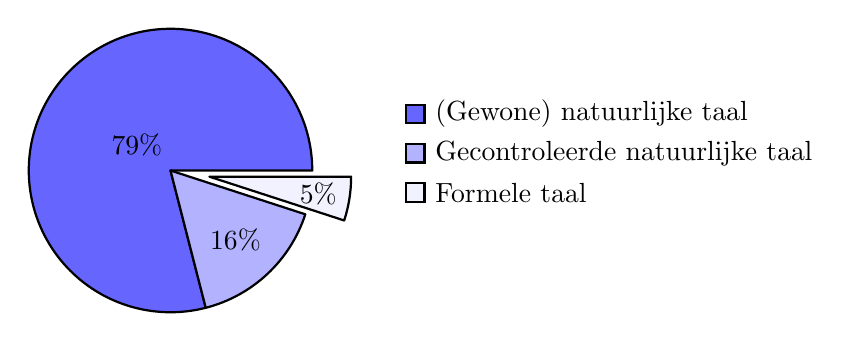
\begin{tikzpicture}
      \pie[text = legend, radius = 1.8, explode = {0, 0, 0.5}, color = {blue!60, blue!30, blue!5}]{79/(Gewone) natuurlijke taal, 16/Gecontroleerde natuurlijke taal, 5/Formele taal}
  \end{tikzpicture}
  \caption[Gebruik van natuurlijke taal in vereistenanalyse]{Gebruik van natuurlijke taal in vereistenanalyse in 1999 (van figuur 5 in \cite{Luisa2004})}
  \label{fig:natural-language-use}
\end{figure}

\paragraph{} We voeren ons onderzoek naar zo'n formele natuurlijke taal uit binnen het domein van logigrammen. Ze kunnen namelijk aanzien worden als kleine specificaties. Bovendien kunnen ze uitgedrukt worden in relatief simpele logische zinnen. Ten slotte kan men makkelijk vele voorbeelden vinden van zo'n logigrammen. We zullen hierbij zelf geen grammatica opstellen maar een aantal grammaticale regels afleiden van bestaande logigrammen (uit Puzzle Baron's Logic Puzzles Volume 3 \cite{logigrammen}).


% Nu begint de eigenlijke tekst
\mainmatter
\chapter{Achtergrond}
Om deze thesis te begrijpen worden hier een aantal concepten uitgelegd die niet per se tot de achtergrondkennis behoren van de lezer. Definite Clause Grammars zijn een soort van grammatica die een aantal voordelen biedt voor het parsen van natuurlijke taal. Feature structures zorgen voor een beperking van het aantal grammaticale regels en verhogen de leesbaarheid ervan. Discourse Representation Theory is een theorie uit de taalkunde voor het vatten van de betekenis van taal. Het introduceert Discourse Representation Structures, een logica die dichter aanleunt bij de natuurlijke taal.

\section{Definite Clause Grammars}
\label{sec:DCG}
Definite Clause Grammars \cite{Pereira1980} zijn een uitbreiding van contextvrije grammatica's die vaak ingebakken zitten in logische talen zoals prolog. Pereira et al.\ \cite{Pereira1980} geven 3 voorbeelden van hoe DCG's kunnen helpen bij het parsen van natuurlijke talen:

\begin{enumerate}
  \item De woordvorm kan afhankelijk gemaakt worden van de context waarin deze verschijnt. Zo kan men eisen dat een werkwoord in de juiste vervoeging voorkomt.
  \item Tijdens het parsen kan men een boom opbouwen die de semantiek van de zin moet vatten. Deze boom hoeft niet isomorf te zijn met de structuur van de grammatica.
  \item Het is mogelijk om prolog code toe te voegen die extra restricties oplegt aan de grammatica.
\end{enumerate}

\subsection{Een eerste grammatica}
\begin{ex}
  Een voorbeeld van een DCG grammatica is:
  \begin{quote}
    \texttt{s ---> np, vp.} \\
    \texttt{np ---> [ik].} \\
    \texttt{np ---> [hem].} \\
    \texttt{vp ---> v, np.} \\
    \texttt{v ---> [zie].}
  \end{quote}
\end{ex} 
\texttt{s} is het startsymbool en staat voor \texttt{sentence}. \texttt{np} staat voor \texttt{noun phrase} (naamwoordgroep of nominale constituent), \texttt{vp} voor \texttt{verb phrase} (verbale constituent) en \texttt{v} voor \texttt{verb}. Deze grammatica zegt dat een zin bestaat uit een noun phrase gevold door een verb phrase. Een verb phrase is dan weer een werkwoord gevolgd door een noun phrase.

De zin \example{ik zie hem} is onderdeel van deze taal. Maar ook de zin \example{ik zie ik} is deel van de taal. Om dit op te lossen kunnen we argumenten meegeven aan de niet-terminaal \texttt{np}.

\subsection{De woordvorm is afhankelijk van de context}
\begin{ex}
  \label{ex:nom-acc-features}
  Deze verbeterde grammatica houdt rekening met welke woordvorm kan voorkomen in welke context.
  \begin{quote}
    \texttt{s ---> np(nom), vp.} \\
    \texttt{np(nom) ---> [ik].} \\
    \texttt{np(acc) ---> [hem].} \\
    \texttt{vp ---> v, np(acc).} \\
    \texttt{v ---> [zie].} \\
  \end{quote}
\end{ex} 

De \texttt{nom} en \texttt{acc} slaan hier op de naamvallen \texttt{nominatief} en \texttt{accusatief}. Ze geven aan in welke functie de naamwoordgroepen gebruikt mogen worden binnen een zin.

\subsection{Een boom als resultaat}
\begin{ex} Verder is het ook mogelijk om een boom op te bouwen tijdens het parsen.
  \begin{quote}
    \texttt{s(Tree) ---> np(NP, nom), vp(Tree, NP).} \\
    \texttt{np(ik, nom) ---> [ik].} \\
    \texttt{np(hem, acc) ---> [hem].} \\
    \texttt{vp(Tree, Subject) ---> v(Tree, Subject, Object), np(Object, acc).} \\
    \texttt{v(zien(Subject, Object), Subject, Object) ---> [zie].}
  \end{quote}
\end{ex} 

Bij het parsen van \example{ik zie hem} krijgen we nu volgende boom:

\Tree[.\textit{zien} \textit{ik} \textit{hem} ]

Merk op dat deze boom de structuur van de grammatica niet hoeft te volgen. Het werkwoord wordt hier tot belangrijkste woord van de zin gebombardeerd.

\subsection{Prolog-code in de grammatica}
\begin{ex} Ten slotte is het mogelijk om prolog restricties te embedden in de grammatica door deze prolog goals tussen accolades te plaatsen.
  \begin{quote}
    \texttt{expression(X) ---> factor(X).} \\
    \texttt{expression(X) ---> term(X).} \\

    \texttt{factor(X) ---> numeral(X).} \\
    \texttt{factor(X) ---> numberal(A), [*], factor(B), \{X is A * B\}.} \\
    \texttt{term(X) ---> factor(A), [+], expression(B), \{X is A + B\}.} \\

    \texttt{numeral(X) ---> [X], \{number(X)\}.} \\
  \end{quote}
\end{ex} 

Bovenstaande grammatica kan simpele wiskunde expressies omvormen tot de wiskundige waarde. Zo wordt \texttt{2 + 4 * 5} omgevormd tot \texttt{22} volgens volgende boom. Hierbij wordt de waarde van onder uit de boom naar boven toe gepropageerd via unificatie.

\Tree[.expression(22)
        [.term(22) [.factor(2) [.number(2) 2 ]]
                   +
                   [.expression(20) [.factor(20) [.number(4) 4 ] * [.factor(5) [.number(5) 5 ]]]]]]

De prologcode in de accolades heeft twee functies. Enerzijds berekent die de waarde van een subexpressie zoals een factor of een term. Anderzijds beperkt de prologcode de grammatica. Een \texttt{numeral} bestaat uit 1 token maar enkel als dat token een getal is volgens prolog. Zo'n beperking in prolog kan ook gebruikt worden om uit de beperkingen van een contextvrije grammatica te treden.

\subsection{Conclusie}
\paragraph{} Definite Clause Grammars zijn expressieve grammatica's die uitermate geschikt zijn voor het modelleren van de grammatica van een natuurlijke taal. In deze thesis zullen alle grammatica's dan ook gegeven worden in de vorm van een DCG.

% \paragraph{}Een laatste opmerking bij deze grammatica is de asymmetrische vorm voor factoren en termen. Een factor is bijvoorbeeld niet gedefinieerd als de vermenigvuldiging van 2 factoren. Dit komt omdat DCG's niet enkel definities zijn van grammatica's maar ook een uitvoeringsstrategie hebben. M.a.w. men krijgt er gratis een parser bij. Deze parser werkt, net als prolog, top-down en van links naar rechts. In het geval van links recursieve regels, zou de parser in een oneindige lus kunnen geraken. Het is echter een bekend resultaat dat men een grammatica altijd kan omvormen zodat deze niet langer links recursief is. Dit is dus geen beperking op welke talen voorgesteld kunnen worden.

% \paragraph{} DCG's zonder prolog code zijn zeer declaratief. Men kan ze namelijk ook puur als definitie van een grammatica beschouwen. Zo kan men een chart parser schrijven die gebruik maakt van een DCG als definitie van de grammatica. Chart parsers zijn interessant voor CNL's omdat ze onthouden welke parti\"ele en volledige constituenten ze al gevonden hebben \cite{Kuhn2008}. Daardoor is er geen nood aan backtracking. Men moet zo niet telkens opnieuw bewijzen wat in een andere tak al bewezen was. Een chart parser onthoudt dat \example{een man} een naamwoordgroep is en kijkt hoe het deze woordgroep kan combineren met andere woorden tot parti\"ele of volledige constituenten. Daardoor is een chart parser veel sneller dan de gratis parser van prolog.

% Bovendien kan men uit de parti\"ele constituenten afleiden welke woordcategorie\"en kunnen volgen op een parti\"ele zin. Zo kan de parti\"ele zin \example{Een rode} gevolgd worden door een adjectief of substantief maar niet door een lidwoord of een werkwoord. Op basis hiervan kan men een suggestietool maken die suggesties geeft i.v.m.\ welke woorden kunnen volgen.

% Ten slotte kan men bij het toevoegen van een woord aan een parti\"ele zin, de resultaten van de vorige parse gebruiken. Dit levert een extra performantiewinst op t.o.v.\ de gratis parser in het geval van incrementele parses. Dit is vooral interessant tijdens het schrijven van een zin, waarbij de vorige parti\"ele zin steeds wordt uitgebreid met \'e\'en woord. Een chart parser hoeft in dat geval namelijk enkel te kijken naar dit nieuwe woord en naar wat er in het geheugen is van de vorige parse, niet meer naar de andere woorden in de zin.

\section{Feature structures}
\label{sec:featureStructures}

\paragraph{} Een feature structure is een term uit de taalkunde. Men kan ze zien als \textit{named arguments} voor een niet-terminaal die gebruikt worden om een explosie aan grammaticale regels te voorkomen. Zo kan een \texttt{np} en \texttt{vp} een feature \texttt{getal} hebben dat aangeeft of de woordgroep in het enkelvoud of meervoud staat. De grammaticale regel voor een zin kan dan aangeven dat het onderwerp en werkwoord moeten overeenkomen in getal. Andere features geven bijvoorbeeld de naamval aan van een naamwoordgroep. Blackburn en Striegnitz \cite{NLPCourse} geven de volgende grammaticale regel als voorbeeld (hierbij staat \texttt{CAT} voor de categorie van een woordgroep):

\[
  \fstructure{
    \feature{CAT}{s}
  }
  \rightarrow
  \fstructure{
    \feature{CAT}{np}
    \feature{NAAMVAL}{nom}
    \feature{GETAL}{\fvariable{1}}
  }
  \fstructure{
    \feature{CAT}{vp}
    \feature{GETAL}{\fvariable{1}}
  }
\]

Deze regel zegt dat een zin bestaat uit een \texttt{np} gevolgd door een \texttt{vp}. De \texttt{np} moet de naamval \texttt{nom} (nominatief) hebben. Bovendien moet het getal van de \texttt{np} en de \texttt{vp} unificeren (de \framebox{1} is een variabele).

Grammatica's die gebruik maken van feature structures, gebruiken altijd unificatie voor het samenvoegen van meerdere structuren. Niet alle features moeten namelijk altijd een waarde toegekend krijgen. Zo kan een eigennaam voorkomen als onderwerp en als lijdend voorwerp (en heeft dus geen waarde voor de feature \texttt{naamval}). Terwijl \example{ik} enkel als onderwerp kan voorkomen (en dus wel een waarde heeft voor die feature). Zoals in het voorbeeld hierboven kan men door unificatie ook controleren of meerdere woordgroepen dezelfde waarden hebben voor een feature.

\paragraph{} Zoals Shieber et al.\ \cite{Shieber2003} aanhalen, verschillen prolog termen van feature structures enkel in vorm. Zo speelt de volgorde in prolog wel een rol. Bovendien moet men steeds alle features vermelden, ook als ze ongebonden zijn. Qua expressiviteit voegen ze echter niets toe aan DCG's. Zo is bovenstaande grammaticale regel op basis van feature structures equivalent met volgende DCG-regel:

\[
    \texttt{s ---> np([naamval:nom, getal:Getal]), vp([getal:Getal]).} \\
\]

\paragraph{} Feature structures (en argumenten in DCG's) zijn handig om de explosie van grammatica regels te voorkomen.
\begin{ex}  Een voorbeeld van een grammatica zonder feature structures (uit \cite{NLPCourse}):
  \label{ex:explosion}
  \begin{quote}
    \texttt{s ---> np\_{singular}, vp\_{singular}.} \\
    \texttt{s ---> np\_{plural}, vp\_{plural}.} \\
    \texttt{np ---> np\_{singular}.} \\
    \texttt{np ---> np\_{plural}.} \\
    \texttt{np\_{singular} ---> det, n\_{singular}.} \\
    \texttt{np\_{plural} ---> det, n\_{plural}.} \\
    \texttt{vp\_{singular} ---> intransitive\_verb\_{singular}.} \\
    \texttt{vp\_{singular} ---> transitive\_verb\_{singular}, np.} \\
    \texttt{vp\_{plural} ---> intransitive\_verb\_{plural}.} \\
    \texttt{vp\_{plural} ---> transitive\_verb\_{plural}, np.} \\
    \texttt{n\_singular ---> [man].} \\
    ...
  \end{quote}
\end{ex} 
Hierbij staat de \texttt{n} voor zelfstandig naamwoord (van het Engelse \texttt{noun}) en \texttt{det} voor determinator. Deze grammatica can veel korter gemaakt worden door gebruik te maken van feature structures:

\begin{ex}  Een grammatica met feature structures equivalent aan voorbeeld \ref{ex:explosion} (ook uit \cite{NLPCourse})
  \begin{quote}
    \texttt{s ---> np([num:Num]), vp([num:Num]).} \\
    \texttt{np([num:Num]) ---> det, n(num:Num).} \\
    \texttt{vp([num:Num]) ---> intransitive\_verb([num:Num]).} \\
    \texttt{vp([num:Num]) ---> transitive\_verb([num:Num]), np(\_).} \\
    \texttt{n([num:singular]) ---> [man].} \\
    ...
  \end{quote}
\end{ex} 

\paragraph{Conclusie} Door gebruik te maken van feature structures is de grammatica simpeler en leesbaarder. Bovendien hoeft het concept dat een zin bestaat uit een \texttt{np} gevolgd door een \texttt{vp} maar \'e\'en keer te worden uitgedrukt. De feature structures zorgen voor de congruentie in getal van het onderwerp met het werkwoord.

\section{Discourse Representation Theory}
Voor het vertalen van natuurlijke taal naar logica zouden we graag gebruik maken van Frege's compositionality principe: De betekenis van een zin bestaat uit de combinatie van de betekenissen van de delen ervan. Als we eerste-orde-logica als doeltaal van onze vertaling nemen, komen we echter vrij snel in de problemen. Neem bijvoorbeeld de zin ``If a man lives, he breathes''. De vertaling hiervan in eerste-orde-logica is $\forall x. man(x) \Rightarrow breathes(x)$. De vertaling van ``a man lives'' is echter $\exists x. man(x)$, wat geen deel uit maakt van de betekenis van de hele zin. Blackburn en Bos \cite{Blackburn2006} geven nog een aantal andere voorbeelden waarvoor DRS-structuren beter geschikt zijn dan eerste-orde-logica (bijvoorbeeld voor het oplossen van anaforische referenties).

Ze suggereren Discourse Representation Structures als alternatief. Deze structuren bestaan uit een lijst van \textit{discourse referents} (woordgroepen waarnaar andere woordgroepen kunnen verwijzen) en een lijst van condities i.v.m. die referenties \cite{Bos2011}. Blackburn en Bos \cite{Blackburn2006} geven o.a. een vertaling van deze DRS-structuren naar eerste-orde-logica. DRS-structuren hebben dus ook een formele betekenis, zoals we verder zullen aantonen, zijn ze echter beter geschikt als doeltaal. Van hieruit kan dan verder vertaald worden naar eerste-orde-logica volgens de vertaling van Blackburn en Bos. Wij hernemen hier hun vertaling als verdere introductie tot deze structuren:

\[
  \Bigg(\drs{x_1, \ldots, x_n}{
      \gamma_1 \\
      \ldots \\
      \gamma_m
    }\Bigg)^{fo} = \exists x_{1} \ldots \exists x_n\Big((\gamma_{1})^{fo} \land \ldots \land (\gamma_m)^{fo}\Big)
\]

En de vertaling van alle mogelijke condities $\gamma$:

\[\Big(R(x_1, ..., x_n)\Big)^{fo} = R(x_1, ..., x_n)\]
\[\Big(\tau_1 = \tau_2\Big)^{fo} = \Big(\tau_1 = \tau_2\Big)\]
\[\Big(\lnot B)^{fo} = \lnot\Big(B\Big)^{fo}\]
\[\Big(B_1 \lor B_2)^{fo} = \Big(B_1\Big)^{fo} \lor \Big(B_2\Big)^{fo}\]

\[\Big(\drs{x_1, ..., x_n}{\gamma_1 \\ ... \\ \gamma_m} \Rightarrow B\Big)^{fo} =  \forall x_1...\forall x_n\Bigg(\Big((\gamma_1)^{fo} \land ... \land (\gamma_m)^{fo}\Big) \Rightarrow \Big(B\Big)^{fo} \Bigg)\]

Ten slotte kan men twee DRS-structuren samenvoegen door de referenties en de condities samen te voegen:

\[
  \drsMerge{\drs{x_1, \ldots, x_k}{
      \gamma_1 \\
      \ldots \\
      \gamma_l
    }}{\drs{y_1, \ldots, y_m}{
      \delta_1 \\
      \ldots \\
      \delta_n
    }} = \drs{x_1, \ldots, x_k, y_1, \ldots, y_m}{
    \gamma_1 \\
    \ldots \\
    \gamma_l \\
    \delta_1 \\
    \ldots \\
    \delta_n
  }
\]

De vertaling van ``If a man lives, he breathes'' naar DRS is \\

\drs{}{\ifdrs{x}{man(x) \\ lives(x)}{}{breathes(x)}}

\paragraph{} Merk op dat de betekenis van het deel ``a man lives'' \drs{x}{man(x) \\ lives(x)} wel deel uitmaakt van de betekenis van de hele zin.

\section{Conclusie} Definite Clause Grammars vormen een expressieve grammatica die natuurlijke taal in al haar facetten makkelijk kan modelleren. Feature Structures komen overeen met argumenten in prolog en kunnen gebruikt worden om grammatica's kort en leesbaar te houden. Discourse Representation Structures vormen een representatie die tussen natuurlijke taal en eerste-orde-logica ligt. Ze zijn even expressief als eerste-orde-logica maar een aantal concepten in de natuurlijke taal zijn beter te modelleren met DRS-structuren.


\chapter{Eerder werk}
\label{ch:related}
In het verleden zijn er al meerdere CNL's gemaakt. Sommige zijn ontworpen om de leesbaarheid van de specificaties te verhogen en hebben geen formele semantiek. Daarom heeft Kuhn \cite{Kuhn2014} een classificatieschema ontwerpen voor CNL's genaamd PENS: \texttt{Precision} (hoe ambigu/formeel is de taal), \texttt{Expressivity} (welke problemen kunnen we uitdrukken), \texttt{Naturalness} (hoe vlot leest de taal), \texttt{Simplicity} (hoe simpel is de taal). In dezelfde paper lijst Kuhn ook een heleboel CNL's op met hun geschiedenis en nut alsook hun classificatie volgens het PENS-schema.

Meer in het algemeen is het omvormen van teksten in natuurlijke taal tot formele modellen al gebeurd in verschillende domeinen: in vereistenanalyse, in het paradigma van business rules, binnen de computationele lingu\"istiek en ten slotte in het domein van de kennisrepresentatie.

Deze sectie geeft een kort overzicht van wat er al gebeurd is in al deze domeinen. Voor een completer overzicht van CNL's, verwijzen we naar Kuhn \cite{Kuhn2014}.

\section{Vereistenanalyse}
\paragraph{Circe} De tool Circe \cite{Ambriola1997} wordt gebruikt in vereistenanalyse. De gebruiker moet een vocabularium, een set van substitutieregels en een specificatie in natuurlijke aanleveren. De tool probeert dan steeds de beste substitutieregel te vinden om zo de tekst geleidelijk aan te transformeren naar een formeel model. Het grote voordeel van de methode is dat er regelsets bestaan voor meerdere soorten modellen: data flow modellen, entity-relationship modellen, ...

Verder is het in Circe mogelijk om in het vocabularium woorden te taggen. De regels kunnen hier dan gebruik van maken om te bepalen of ze van toepassing zijn op bepaalde zinnen. Op die manier introduceert Circe types in het vocabularium.

Een voorbeeld (uit \cite{Ambriola1997}): \example{bron/UIT STUURT data/INFO NAAR doel/IN}. De woorden \example{stuurt} en \example{naar} liggen vast in de regelset. De andere 3 woorden komen uit het vocabularium. Deze moeten een bepaalde tag hebben om te matchen met de regel. Er zijn dus drie types in deze zin: entiteiten die informatie kunnen versturen, entiteiten die informatie kunnen ontvangen en informatie die verzonden kan worden.

Circe is niet echt een CNL. Zinnen die niet matchen met een substitutieregel worden ook niet omgezet in een formeel model. De specificatie kan dus zinnen met en zonder formele betekenis mengen. Er is geen sprake van constructieregels. Alleen (delen van) zinnen die matchen met een substitutieregel krijgen een formele betekenis.

\section{Business rules}
Binnen het paradigma van business rules spelen zowel natuurlijke talen als formele talen een grote rol. SBVR Structured English (SBVR-SE) \cite{Levy2013} en RuleSpeak \cite{Ross2009a} zijn 2 CNL's die proberen om ambigu\"iteit in de natuurlijke taal te verminderen. Deze talen focussen echter vooral op het menselijke aspect \cite{Njonko2014}. Het doel van deze talen is om ambigu\"iteit uit de specificatie te halen en niet zozeer om automatisch natuurlijke taal om te zetten naar een formele voorstelling. RuleCNL \cite{Njonko2014} heeft wel dit doel.

RuleCNL splitst de specificatie op in twee delen: een vocabularium en de regels zelf. Het vocabularium bestaat uit substantieven en werkwoorden alsook hoe deze in verhouding staan tot elkaar. Bijvoorbeeld \example{Auto heeft wiel} geeft aan dat er een relatie kan bestaan tussen een auto en een wiel. Het vocabularium in RuleCNL is dus getypeerd. Voor de regels zelf bestaat er een contextvrije grammatica waaraan de zinnen moeten voldoen.

Om de gebruikers te helpen bij het schrijven van de zinnen in RuleCNL, is er een plug-in voor de Eclipse IDE die automatisch zinnen kan aanvullen en de structuur van bestaande zinnen aangeeft door het kleuren ervan. Bovendien is er een visuele representatie van het domein om de gebruiker te helpen bij het schrijven van het vocabularium.

\section{Computationele lingu\"istiek} Er zijn reeds 2 belangrijke CNL's opgesteld die vertaald kunnen worden naar formele modellen: Attempto Controlled English (ACE) en Processable English (PENG). Beide talen lijken op elkaar en hebben gelijkaardige tools om mee te werken. Ze komen ook allebei uit de computationele lingu\"istiek en zijn ingebakken in taalkundige frameworks die gemaakt zijn om de semantiek van natuurlijke taal in het algemeen te vatten. In de papers over ACE en PENG wordt er niet zoveel gesproken over deze taalkundige aspecten omdat een achtergrond in de (computationele) lingu\"istiek verondersteld wordt.

Hierna volgt eerst een bespreking van ACE. Daarna bespreken we PENG. Hierbij ligt de nadruk op de gelijkenissen en verschillen met ACE. We sluiten af met een beschrijving van hoe deze twee talen ge\"implementeerd zijn met een nadruk op de verduidelijking van een aantal taalkundige aspecten die amper aan bod komen in de papers over ACE en PENG.

\subsection{Attempto Controlled English (ACE)}
\paragraph{} Attempto Controlled English \cite{Fuchs2008} is een gecontroleerde natuurlijke taal voor kennisrepresentatie. Het is een subset van Engels die naar een subset van eerste-orde-logica vertaalt. Het is een formele taal: elke zin in ACE heeft slechts \'e\'en betekenis, ook al is de zin ambigu in het Engels. Om te bepalen welke van de betekenissen de \textit{correcte} betekenis is, moet men de interpretatieregels volgen. Omdat dit soms nogal ingewikkeld is, kan men gebruik maken van de parafraseertool van ACE. Deze tool zet de interne representatie terug om naar \'e\'en of meerdere zinnen in ACE. Op die manier kan men niet alleen de betekenis van de zin leren, maar ook de taal zelf. Deze parafrasering leunt echter zeer nauw aan bij de formele taal. Hierdoor is ze niet altijd toegankelijk voor iemand zonder een achtergrond in formele talen.

Bijvoorbeeld de zin \example{Everybody is not present.} heeft 2 betekenissen in het Engels: \example{Everybody is absent} en \example{Somebody is absent}. In ACE is de eerste betekenis de \textit{correcte}. Deze zin wordt geparafraseerd als \example{If there is somebody X1 then it is false that X1 is present.}\footnote{De parafrasering komt van de Attempto Parsing Engine (http://attempto.ifi.uzh.ch/ape/)}. Dit is al een vrij moeilijke parafrasering om te begrijpen terwijl de originele zin nog redelijk simpel is.

\paragraph{}ACE is een general purpose CNL: Het bevat een ingebouwd vocabularium. De gebruiker moet dus zelf geen vocabularium opstellen en kan direct beginnen met het schrijven van de specificatie. Het nadeel aan deze aanpak is dat ACE dus ook geen domeinkennis kan gebruiken voor het analyseren van de zinnen. Sommige constructies moeten daarom met een koppelteken geschreven worden. Zo wordt er in \cite{ACEConstructionRules} het voorbeeld gegeven van \example{A student is interested-in a course} en \example{A student is interested in a classroom}.

Op die manier probeert ACE sommige ambigu\"iteiten op te lossen. Een gelijkaardige truc wordt bijvoorbeeld ook gebruikt om de voorrang van \example{en} en \example{of} op te lossen. Standaard heeft \example{en} voorrang. Maar als de \example{en} voorafgegaan wordt door een komma, dan heeft \example{of} voorrang. \cite{ACEConstructionRules} geeft het voorbeeld \example{A client \{enters a red card or enters a blue card\}, and enters a code.}

In andere gevallen kiest ACE gewoon hoe de zin ge\"interpreteerd moet worden op basis van een set van interpretatieregels. Zo slaat de \example{manually} in \example{A customer who {enters a card manually} types a code.} \cite{ACEConstructionRules} op \example{enters} en niet op \example{types} omdat een bijwoord bij voorkeur achter het werkwoord staat. (De parafrasering is in dit geval wel makkelijk te begrijpen maar vrij lang: \example{There is a customer X1. The customer X1 types a code. The customer X1 enters a card manually.}). Merk ook op dat het onbepaalde lidwoord aanleiding geeft tot een existenti\"ele quantor. In dit geval is de universele quantor echter beter geschikt.

\paragraph{} \'E\'en van de sterke punten van ACE is haar coreferentie-analyse. Dit is het onderzoeken van welke woordgroepen naar hetzelfde concept verwijzen. Neem bijvoorbeeld de zinnen \example{Een man heeft een vrouw. Hij is gelukkig.}. Hierin is \example{Hij} een anaforische referentie (een referentie naar een woordgroep die eerder komt) naar \example{een man}. ACE kan deze coreferenties correct analyseren. ACE doet dit door haar embedding in Discourse Representation Theory, een taalkundig framework. Men kan hier redelijk ver in gaan. Zo worden de zinnen \example{There is a red house and there is a blue house. The red house is large.} correct geanalyseerd. Doordat zinnen in ACE als \'e\'en geheel vertaald worden, kan men dus lange zinnen met veel bijzinnen herschrijven in meerdere kortere zinnen. Dit kan de leesbaarheid van een specificatie vergroten.

\paragraph{} Origineel was ACE bedoeld voor het opstellen van specificaties voor software. Ondertussen kent de taal al meerdere toepassingen, in verschillende domeinen. Er zijn ook meerdere tools die overweg kunnen met ACE als input.

Zo is er de Attempto Parsing Engine APE die ACE zinnen omzet naar Discourse Representation Structures. Dit zijn datatypes uit Discourse Representation Theory die de semantiek van de zin bevatten. APE geeft ook een parafrasering van de invoertekst. Zodat de gebruiker kan controleren of de tool de tekst op de juiste manier leest. Bovendien kan APE waarschuwingen geven bij mogelijke problemen. Bijvoorbeeld het gebruik van een anaforische referentie zonder een antecedent waarnaar deze anafoor kan verwijzen.

\paragraph{} Verder is er de Attempto Reasoner RACE. Deze tool kan controleren of een specificatie consistent is. Indien niet, zal de tool zeggen welke zinnen met elkaar in conflict zijn. Op die manier weet de gebruiker dat er een fout is en waar deze zich ongeveer bevindt. Daarnaast kan de tool vragen in natuurlijke taal beantwoorden. RACE antwoordt niet alleen op de vraag maar geeft ook de zinnen die nodig zijn om te bewijzen dat het gegeven antwoord juist is. Ten slotte kan RACE bewijzen of een bepaalde zin het logische gevolg is van de specificatie. Op die manier kan de gebruiker testen of de specificatie correct is.

APE en RACE zijn de twee belangrijkste tools. Er zijn er echter nog veel meer. Zo is er de ACE View Prot\'eg\'e plug-in. Dit is een plug-in die de vertaling tussen Web Ontology Language (OWL) en ACE doet binnen de Prot\'eg\'e-omgeving (een editor voor het maken van ontologi\"en). Op die manier ziet de gebruiker enkel ACE zinnen en hoeft dus de formele OWL taal niet te kennen om met bestaande modellen om te gaan of om nieuwe modellen te maken. Ten slotte is er AceRules. Hiermee kan de gebruiker de zinnen die ge\"impliceerd worden door de specificatie te weten komen.

Over het algemeen is ACE een zeer uitgebreide taal. Veel Engelse zinnen zijn geldige ACE zinnen, echter niet allemaal. Hierdoor is het moeilijk om de taal te leren. Het is immers niet super duidelijk wat toegestaan is en wat niet. Volgens Fuchs et al.\ \cite{Fuchs2008} heeft een gebruiker 2 dagen nodig om de taal te leren.

\subsection{Processable English (PENG)}
\paragraph{} Andere talen zoals PENG \cite{Schwitter2002} zijn makkelijker om te leren dan ACE. PENG is net als ACE een CNL die vertaalt naar DRS-structuren. In tegenstelling tot ACE bevat PENG geen groot ingebouwd lexicon. De gebruiker moet zelf de woorden aanbrengen die gebruikt worden. De gebruiker kan dit doen tijdens het bewerken en moet dus niet op voorhand aangeven wat het lexicon is. De categorie\"en voor deze domeinspecifieke woorden zijn substantief, adjectief, werkwoord of bijwoord. PENG biedt ook de mogelijkheid om synoniemen of afkortingen te introduceren. Op die manier kan de specificatie vlotter gemaakt worden. Men kan echter geen types meegeven in het lexicon. Men kan dus niet zeggen dat het werkwoord \example{ademen} enkel uitgevoerd kan worden doormensen of dieren en niet door objecten. Naast de domeinspecifieke woorden kent PENG een aantal functionele woorden die ingebakken zitten in de taal, zoals lidwoorden en voegwoorden (\example{de man \underline{die}}). Deze woorden helpen PENG om de zinsconstructies te herkennen.

Net zoals ACE kent PENG het principe van constructieregels en interpretatieregels. De constructieregels bepalen welke zinnen deel zijn van de taal. Bij PENG zijn deze regels eenvoudiger omdat de taal zeer simpel gehouden is. Hierdoor is het makkelijker om zinnen te maken in de taal. Over het algemeen lijken de constructieregels van PENG en ACE veel op elkaar.

De interpretatieregels bepalen hoe de zin vertaald wordt naar logica. Zo is er een interpretatieregel voor hoe anaforische referenties opgelost worden. Deze regel is gelijkaardig in ACE en PENG. Andere regels bepalen welke functiewoorden sterker binden. Zowel ACE als PENG gebruiken hiervoor dezelfde volgorde als in eerste-orde-logica. ACE staat wel uitzonderingen toe door het toevoegen van komma's. PENG houdt de taal simpel en staat dit niet toe.

\paragraph{} PENG is makkelijker om te leren dan ACE omwille van ECOLE \cite{Schwitter2003}. Een tool die suggesties geeft over de woordcategorie\"en die kunnen volgen op een bepaalde zin. Zo geeft Schwitter \cite{Schwitter2003} het voorbeeld van \example{Een} dat gevolgd kan worden door een \texttt{adjectief} of een \texttt{substantief}. Indien de gebruiker de woordcategorie niet kent, kan hij doorklikken op die categorie voor een aantal concrete mogelijkheden. Op die manier moet de gebruiker enkel de woordcategorie\"en leren en niet de geldige zinsconstructies.

Naast de suggestietool bestaat er voor PENG, net zoals voor ACE, ook een parafraseertool. Deze tool herschrijft de invoer zodat het duidelijker is hoe PENG de zin begrepen heeft. Anaforische referenties worden bijvoorbeeld omgezet in de naamwoordgroep waarnaar ze verwijzen.

Net zoals voor ACE zinnen is het ook voor een PENG zinnen mogelijk om te controleren of ze een consistente specificatie vormen \cite{Schwitter2004b}. Daarnaast is het mogelijk om te controleren op redundantie. Indien een zin al door een andere zin ge\"impliceerd wordt, hoeft deze niet expliciet deel uit te maken van de specificatie. Op die manier kan de specificatie kort gehouden worden, wat de leesbaarheid verhoogd.

Naast de general purpose CNL bevat PENG ook een subset specifiek voor het semantische web: PENG-D \cite{Schwitter2004}. Deze subset kan vertaald worden naar description logic (OWL DL), een subset van eerste-orde-logica. PENG-D kan dus gezien worden als het alternatief voor de ACE View Prot\'eg\'e plug-in.
Schwitter \cite{Schwitter2006} vermeldt drie klassieke manieren van voorstellen van een ontologie (N-Triples, RDF/XML en OWL Abstract) en toont dan verder aan dat PENG een vierde manier is om hetzelfde voor te stellen. De paper toont dit aan door verschillende constructies uit OWL te mappen op zinnen in PENG. Het grote voordeel van PENG t.o.v. de andere voorstellingswijzen is dat PENG ook leesbaar en begrijpbaar is voor de mens.

\subsection{Implementatie}
\paragraph{} Zowel ACE als PENG zijn ge\"implementeerd in prolog met behulp van Definite Clause Grammars (DCG) en feature structures voor het omzetten van de natuurlijke taal naar DRS-structuren \cite{Fuchs2008, Schwitter2006}.

\paragraph{Definite Clause Grammars} Aangezien zowel ACE als PENG gebruiken maken van prolog voor hun (eerste) implementatie, is de keuze voor DCG's voor de hand liggend omwille van de parser die men er gratis bijkrijgt. In de tools voor ACE en PENG wordt er echter gebruik gemaakt van een chart parser. Deze parser kan tijdens het schrijven van de zinnen, heel snel voorspellen welke woordcategorie\"en kunnen volgen. Dit helpt de gebruiker bij het schrijven van grammaticaal correcte zinnen zonder de taal te moeten kennen. PENG gebruikt zo'n chart parsers in ECOLE \cite{Schwitter2003}. ACE heeft in navolging van PENG ook AceWiki \cite{Kuhn2008} gemaakt, een subset van ACE voor semantische wiki's. Ook AceWiki bevat een suggestietool. Kuhn et al.\ \cite{Kuhn2008} leggen in detail uit hoe zo'n chart parser gemaakt kan worden voor een CNL en vergelijken de performantie van deze parsers met de gratis parser van prolog.

\paragraph{Feature structures} Binnen DCG's wordt er in ACE en PENG ook veelvuldig gebruikt gemaakt van feature structures \cite{Shieber2003, NLPCourse} \footnote{ACE gebruikt bijvoorbeeld een uitbreiding op prolog genaamd ProFIT \cite{Erbach1995} die deze structuren beter ondersteunt}. Binnen ACE en PENG zorgen de feature structures voor de syntactische correctheid van de zinnen in de gasttaal, het Engels. Via unificatie kan men namelijk testen of een bepaalde woordgroep voldoet aan de voorwaarden van de context. De unificatie van de feature \texttt{getal} van het onderwerp en het werkwoord zorgt voor de congruentie in getal van het onderwerp met het werkwoord. Op die manier zijn zinnen die in ACE en/of PENG geldig zijn, ook geldig in het Engels. Zoals sectie \ref{sec:featureStructures} aanhaalt, wordt op deze manier een explosie van het aantal grammaticale regels vermeden.

\paragraph{DRS} Naast feature structures maken ACE en PENG ook gebruik van Discourse Representation Structures. Ze zijn een onderdeel van Discourse Representation Theory. Dit is een taalkundig framework om de semantiek van natuurlijke taal te vatten. Één van de sterke punten van DRS-structuren is het oplossen van coreferenties. \cite{Fuchs2008drs} bevat meer informatie over hoe DRS-structuren gebruikt worden binnen ACE.

Bos \cite{Bos2011} stelt dat DRS-structuren zowel de rol van semantische inhoud als die van tekstuele context spelen. M.a.w.\ met behulp van deze structuren kan men achterhalen wat de semantiek van een tekst is maar tegelijk bieden ze ook een context aan die helpt bij de coreferentie-analyse. Zo wordt tijdens het parsen de semantiek van een zin opgebouwd en tegelijk de coreferenties opgelost.

Concreet definieert Bos \cite{Bos2011} een DRS-structuur als een lijst van \textit{discourse referents} (woordgroepen waarnaar andere woordgroepen kunnen verwijzen) en een lijst van bepaling i.v.m. die referenties. DRS~\ref{drs:example} geeft een voorbeeld van zo'n DRS-structuur voor de zin \example{There is a movie which every man loves deeply}. Er zijn in totaal 3 \textit{discourse referents}: \texttt{A} (de film), \texttt{B} (de man) en \texttt{C} (het houden van). Merk op dat naar deze laatste verwezen wordt door het bijwoord \textit{deeply}. Deze DRS kan vertaald worden als $\exists A \cdot \bigg(movie(A) \land \forall B \cdot \Big(man(B) \Rightarrow \exists C \cdot \big( loves(C, B, A) \land deeply(C) \big)\Big)\bigg)$

\begin{savenotes}
  \begin{drsFloat}
    \centering
    \drs{A}{
      movie(A) \\
      \ifdrs{B}{man(B)}
            {C}{loves(C, B, A) \\ deeply(C)}
    }
    \caption{Een DRS-structuur voor de zin \example{There is a movie which every man loves deeply.} \protect\footnotemark}
    \label{drs:example}
    \footnotetext{Deze DRS-structuur werd lichtjes aangepast aan de output van APE (http://attempto.ifi.uzh.ch/ape/)}
  \end{drsFloat}
\end{savenotes}


\paragraph{Conclusie} DCG's zijn een uitbreiding op contextvrije grammatica's uit de wereld van logisch programmeren. Feature structures en Discourse Representation Structures zijn concepten uit de lingu\"istiek. Ze worden gebruikt om de natuurlijke taal en haar semantiek te modelleren. Zo helpen feature structures om een explosie van het aantal grammatica regels te voorkomen. Discourse Representation Structures worden dan weer vooral gebruikt om de coreferentie-analyse te vergemakkelijken. Beiden concepten worden gebruikt in de tools rond ACE en PENG omdat deze talen ontstaan zijn in het vakgebied van computationele lingu\"istiek.

\section{Kennisrepresentatie}
\label{sec:ASP}
In het domein van kennisrepresentatie hebben Baral et al.\ \cite{Baral2008} natuurlijke taal reeds vertaald naar Answer Set Programs (ASP). Ze maken hiervoor gebruik van Combinatorische Categorische Grammatica (CCG) en $\lambda$-calcalus. Een CCG bestaat uit een aantal basiscategorie\"en zoals \texttt{s} (zin) en \texttt{np} (naamwoordgroep) en afgeleide categorie\"en zoals \texttt{s/np}\footnote{een \texttt{S/NP} is een woordgroep die indien gecombineerd met een \texttt{np} langs links een zin vormt} en \texttt{(s/np)$\backslash$np}\footnote{een \texttt{(S/NP)$\backslash$NP} is een woordgroep die indien met een \texttt{np} gecombineerd langs links en langs rechts een zin vormt} \cite{Baral2008}. Zo wordt een onovergankelijk werkwoord voorgesteld als een \texttt{s$\backslash$np}. Verder bevat een CCG een aantal regels die bepalen wat de categorie is van een combintatie van woordgroepen. Zo is er een regel die zegt dat $\alpha\beta$ van categorie \texttt{B} is als $\alpha$ categorie \texttt{A} heeft en $\beta$ categorie \texttt{B$\backslash$A} \cite{Baral2008}. Dankzij deze regel kunnen we afleiden dat als we een onovergankelijk werkwoord (\texttt{s$\backslash$np}) langs links combineren met een naamwoordgroep (\texttt{np}), we dan een zin (\texttt{s}) krijgen. Op deze manier kunnen we een parse tree opstellen waarbij we telkens 2 woordgroepen combineren totdat de zin uiteindelijk categorie \texttt{s} krijgt.

Naast een categorie heeft elk woord ook een betekenis uitgedrukt in een uitbreiding op de $\lambda$-calcalus. In deze uitbreiding kunnen ook ASP-expressies voorkomen. De betekenis van een woordgroep is de combinatie van de betekenis van de woorden. Hierbij gebruiken we de CCG parse tree om de volgorde te bepalen. We verduidelijken met een voorbeeld (grotendeels overgenomen uit Baral et al.\ \cite{Baral2008}). We beschouwen het lexicon zoals weergegeven in tabel \ref{table:CCG} voor de zin \example{Birds fly}. De combinatie van de woorden \textit{birds} en \textit{fly}, is van de categorie \texttt{s} zoals hierboven reeds uitgelegd. De overeenkomstige lamda-expressies moeten nu op een gelijkaardige manier gecombineerd worden: $\lambda_{birds\ fly}=\app{\lambda_{fly}}{\lambda_{birds}}$.

\begin{table}
  \centering
  \begin{tabular}{|l|l|l|}
    \hline
    Woord & Categorie & $\lambda$-ASP-expressie \\
    \hline
    \hline
    Birds & np & $\lambda x.bird(x)$ \\
    Fly & s$\backslash$np & $\lambda x.fly(X) \leftarrow \app{x}{X}$ \\
    \hline
  \end{tabular}
  \caption{Een lexicon voor de woorden birds en fly in een CCG grammatica (uit \cite{Baral2008})}
  \label{table:CCG}
\end{table}

\begin{equation}
  \label{eq:lambda}
  \begin{aligned}
  \lambda_{birds\ fly} &= \app{\lambda_{fly}}{\lambda_{birds}} \\
          &= \app{(\lambda x.fly(X) \leftarrow \app{x}{X})}{\lambda x.bird(x)} \\
          &= fly(X) \leftarrow \app{(\lambda x.bird(x))}{X} \\
          &= fly(X) \leftarrow bird(X)
  \end{aligned}
\end{equation}

Elk woord heeft een betekenis die men kan zien als een ASP-expressie met gaten erin die opgevuld worden door de combinatie met andere woorden. De manier van combineren van de $\lambda$-expressies hangt af van de categorie\"en van de woorden. Het nadeel aan deze aanpak is dat elk woord (minstens) \'e\'en betekenis moeten hebben in het formaat van een $\lambda$-ASP-expressie. Constantini et al.\ \cite{Costantini2010} lossen dit probleem deels op door gebruik te maken van $\lambda$-ASP-expressie-templates. Sommige woorden hebben nog steeds een eigen $\lambda$-ASP-expressie, voor de andere kan er \'e\'en afgeleid worden uit een $\lambda$-ASP-expressie-template. Zo is $\lambda x. <noun>(x)$ de template voor substantieven. Het gedeelte $<noun>$ moet vervagen worden door een specifieke instantie. Het woord \textit{birds} heeft zo nog steeds dezelfde betekenis.

\paragraph{}Zo'n templates werken echter niet voor alle woorden. Daarom hebben Baral et al.\ \cite{Baral2012} een methode bedacht om van de betekenis van een zin en de betekenis van een aantal woorden, de betekenis van andere woorden af te leiden. Ze doen dit niet langer met $\lambda$-ASP-expressies maar vervangen ASP door eerste-orde-logica: $\lambda$-FOL-expressies. De grammatica en manier van combineren blijft echter hetzelfde. Deze techniek gebruiken Baral et al.\ \cite{Baral2012a} om automatisch een grammatica en semantiek te leren voor logigrammen op basis van andere logigrammen en hun vertaling in een ASP programma. Hiervoor gebruiken ze \'e\'en ASP-ontologie die toepasbaar is voor vele logigrammen. Ze bewerken hierbij de natuurlijke taal van de logische puzzels een beetje om anaforische referenties te verwijderen. De auteurs benadrukken echter dat dit geen CNL is omdat de grammatica op voorhand niet gedefinieerd is maar geleerd wordt uit de gegeven logische puzzels. Ze maken hiervoor gebruik van een probabilistische CCG. Tot 83\% van de puzzels kunnen ze correct oplossen. De andere puzzels falen o.a.\ omdat bepaalde zinsconstructies niet voorkwamen in de trainingsdata. Belangrijk om op te merken is dat vele woorden (zoals \textit{about}, \textit{on}, \textit{the}) geen betekenis krijgen omdat ze in de logische puzzel geen rol spelen. Er is dus sprake van overfitting op het domein van de logische puzzels.

\paragraph{} Een belangrijk verschil met deze thesis is dat Baral et al. proberen om deze regels automatisch af te leiden, zowel voor de structuur van de grammatica als voor de betekenis van de woorden. Om de techniek uit te breiden naar andere domeinen dan logigrammen, moeten dus nieuwe specificaties eerst manueel gelabeld worden met hun vertaling zodat een vertaling geleerd kan worden die ook van toepassing is op het nieuwe domein.

Bovendien worden KBS-systemen momenteel vooral gebruikt voor mission-critical toepassingen. We willen dus zeker zijn wat de vertaling is van een zin. We zullen daarom geen machine learning technieken gebruiken.

% \chapter{Probleemstelling}
\paragraph{} In deze thesis willen we onderzoeken hoe we een gecontroleerde natuurlijke taal met een eenduidige semantiek kunnen gebruiken voor kennisrepresentatie. We ontwerpen hiervoor een nieuwe taal. De bedoeling is om deze taal toegankelijk te maken voor domein experten, i.e.\ mensen zonder achtergrond in formele talen. Verder bekijken we hoe we deze taal rijk genoeg kunnen maken voor praktische problemen. Ten slotte willen we dat deze taal toepasbaar is binnen het KBS paradigma.

Voor dit laatste willen we daarom, net als RuleCNL, een onderscheid maken tussen het vocabularium (of ontologie) en de theorie (of de regels). Onder het vocabularium verstaan we een modellering van de wereld in concepten en relaties tussen deze concepten. Dit is dus een getypeerd vocabularium, in tegenstelling tot ACE en PENG. We onderzoeken welke extra voordelen dit oplevert. 

Verder onderzoeken we of we uitbreidingen op eerste-orde-logica kunnen integreren in de nieuwe CNL om zo de formele expressiviteit te verhogen. ACE en PENG hebben zich beperkt tot (een subset van) eerste-orde-logica. Het is echter algemeen gekend dat sommige problemen niet uitgedrukt kunnen worden in eerste-orde-logica. Hierdoor zijn deze talen niet altijd rijk genoeg voor praktische problemen.

De focus ligt minder op het ondersteunen van taalkundige constructies zoals anaforische referenties. Dit is reeds grondig onderzocht in ACE en PENG. Verder onderzoek zou eventueel kunnen aantonen hoe die technieken samengebracht kunnen worden met deze thesis.

In tegenstelling tot sectie \ref{sec:ASP} (\nameref{sec:ASP}) is het wel de bedoeling om een taal te construeren en dus een grammatica op te stellen. Op die manier kan de gebruiker de taal ook leren. Door de manuele constructie is de kans op overfitting ook kleiner waardoor deze aanpak ook kan schalen naar nieuwe problemen.

\section{A semantical framework}
Blackburn and Bos constructed a framework~\cite{Blackburn2005, Blackburn2006} to capture the meaning of natural language by translating it into a logic. It consists of four parts: the lexicon, the grammar, the semantics of the lexicon and the semantics of the grammar. The framework is based on the $\lambda$-calculus and Frege's compositionality principle. Every word has an $\lambda$-expression as its meaning. The meaning of a group of words is a combination of the meaning of the words that are part of the group. In this framework, $\lambda$-application will be used to combine words.

The grammar defines which sentences are grammatical and thus allowed and which are not. E.g. a sentence consists of a subject (a noun phrase) and a verb phrase that agree in number. This process results in a parse tree of every grammatical sentence, in which the words are the leaves. The framework then combines the meaning of the leaves (the words) upwards in the tree to the meaning of the root node (the sentence).

\begin{dcg}{A small grammar}{dcg:frameworkIllustration}
s([]) -->
  np([num:Num]),
  vp([num:Num]).
np([num:sg]) -->
  pn([]).
np([num:Num]) -->
  det([]),
  n([num:Num]).
vp([num:Num, sem:Sem]) -->
  iv([num:Num, sem:Sem]).
vp([num:Num, sem:Sem]) -->
  tv([num:Num, sem:]),
  np([num:_]).
\end{dcg}

The lexicon consists of the enumeration of the different words that can be used along with some linguistic features. E.g. ``loves'' is a verb in the present tense, ``love'' is a verb and an infinitive. A lot of words also have a feature \textit{Symbol} which will be used in the translation of the word.

The goal of the framework is to lexicalize as much of the meaning as possible. The semantics of a grammar rule should be limited to $\lambda$-applications, if possible. The most important word of a group of words is then the functor and the other words its arguments. The meaning of a sentence is a $\lambda$-application with the verb phrase as the functor and the noun phrase as the argument, i.e. $\sem{s} = \app{\sem{vp}}{\sem{np}}$. Table~\ref{tbl:grammar-sem} gives the semantics for grammar~\ref{dcg:frameworkIllustration}. The determiner is taken to be the most important word in the noun phrase.

\begin{table}[h]
  \begin{tabular}{@{}ll}
    \hline
    \textbf{Grammatical rule} & \textbf{Semantics} \\
    \hline
    S (line 1-3) & $\sem{s} = \app{\sem{vp}}{\sem{np}}$ \\
    NP1 (line 4-5) & $\sem{np} = \sem{pn}$ \\
    NP2 (line 6-8) & $\sem{np} = \app{\sem{det}}{\sem{n}}$ \\
    VP1 (line 9-10) & $\sem{vp} = \sem{iv}$ \\
    VP2 (line 11-13) & $\sem{vp} = \app{\sem{tv}}{\sem{np}}$\\
    \hline
  \end{tabular}
  \centering
  \caption{De semantics of grammar~\ref{dcg:frameworkIllustration}}
  \label{tbl:grammar-sem}
\end{table}

The meaning of the words is the only thing missing. Blackburn and Bos assume that the meaning of a word is only dependent on its linguistic features, most importantly its linguistic category. Constructing these $\lambda$-expressions can be hard. Therefore, we first analyze the signature of these expressions. We used a $\lambda$-calculus with two types for this: $e$ represents entities and $t$ truth-values. A noun is the easiest. It's signature is $\tau(n) = e \rightarrow t$, given an entity, the noun says whether or not the entity can be described with the noun. A noun phrase represents one or more entities. E.g. ``a man'', ``every woman''. A sentence is true if enough entities of the noun phrase satisfy a certain property of the verb phrase. The signature of a noun phrase is thus $\tau(np) = (e \rightarrow t) \rightarrow t$. Given a property $P$ with signature $e \rightarrow t$, the semantics of the noun phrase will say if enough entities described by the noun phrase, satisfy the property $P$ of the verb phrase. The semantics of the proper noun John is for example $\sem{pn_{John}} = \lambdaf{P}{\app{P}{John}}$. I.e. when we say something about ``John'', the property should hold for $John$. The meaning of the noun phrase ``every man'' is $\sem{np_{every\ man}} = \lambdaf{P}{\forall x \cdot man(x) \Rightarrow P(x)}$. Given a property P, the property should hold for all men for the sentence to be true.

The signature of a verb phrase is $\tau(vp) = \tau(np) \rightarrow \tau(s) = ((e \rightarrow t) \rightarrow t) \rightarrow t$. Given an noun phrase, it should say whether the sentence is true or not. The meaning of the intransitive verb for example is $\sem{iv_{sleeps}} = \lambdaf{S}{\app{S}{\lambdaf{x}{Sleeps(x)}}}$. Given the subject $S$, the sentence is true if the subject holds the property $\lambdaf{x}{Sleeps(x)}$.

The meaning of the sentence ``John sleeps'' is $$\sem{s} = \app{\sem{vp}}{\sem{np}} =$$ $$ \appH{\lambdaf{S}{\app{S}{\lambdaf{x}{Sleeps(x)}}}}{\lambdaf{P}{\app{P}{John}}}$$ $$= Sleeps(John)$$.

% We illustrate the framework using the example ``John sleeps''. John is a proper noun (pn) and sleeps an intransitive verb (iv). The meaning of a proper noun is $\sem{pn} = \lambdaf{M}{\app{M}{Symbol}}$. E.g. $\sem{pn} = \lambdaf{M}{\app{M}{John}}$. This can be read as \textit{given a set-membership function $M$ which represents the entities that execute the verb,  }




\chapter{Lexicon voor logigrammen}
In dit hoofdstuk bespreken we de gebruikte lexicale categorieën. We beperken de categorieën tot een set die het makkelijk maakt voor de vertaling van logigrammen naar DRS-structuren. We bespreken zowel de categorieën zelf alsook hun vertaling naar deze DRS-structuren. Er wordt een onderscheid gemaakt tussen open en gesloten lexicale categorieën. De open categorieën zijn open voor uitbreiding, er kunnen dus woorden aan worden toegevoegd specifiek voor een bepaalde logigram. De gesloten categorieën bevatten woorden die gemeenschappelijk zijn voor alle logigrammen. Tabel~\ref{tbl:lexiconCategories} geeft een overzicht van de gebruikte lexicale categorieën.

\begin{table}[t]
  \centering
  \begin{tabular}{llll}
    \toprule
    \textbf{Categorie} & \textbf{Afkorting} & \textbf{Open?} & \textbf{Voorbeeld}  \\ \midrule
    Determinator       & det                & gesloten & a, an, the \\
    Hoofdtelwoord      & number             & gesloten & three, 5      \\
    Eigennaam          & pn                 & open     & John, ``the black darts'' \\
    Substantief        & n                  & open     & man, year, \\
    Transitief werkwoord & tv               & open     & loves, ``had a final score of'' \\
    Koppelwerkwoord    & cop                & gesloten & is, ``is not'' \\
    Hulpwerkwoord      & av                 & gesloten & does, ``doesn't'' \\
    Betrekkelijk voornaamwoord & relpro     & gesloten & who, which, that \\
    Voorzetsel         & prep               & open     & in, to \\
    Voegwoord          & coord              & gesloten & and, or, ``neither ... nor ...'' \\
    Comparatief        & comp               & open     & above, ``older than'' \\
    \bottomrule
  \end{tabular}
  \caption{Een overzicht van de lexicale categorieën}
  \label{tbl:lexiconCategories}
\end{table}

\section{Determinator}
Een determinator kan zowel een lidwoord als een kwantor zijn. In het geval van logigrammen volstaan de lidwoorden ``a'', ``an'' en ``the''. Deze drie determinatoren krijgen alle drie de vertaling van de existentiële determinator uit het vorige hoofdstuk $$\sem{det} = \sem{det_{existentieel}} = \lambdaf{R}{\lambdaf{S}{\left( \drs{x}{} \oplus \app{R}{x} \oplus \app{S}{x} \right)}}$$ Er is dus geen nood aan een universele of negatieve determinator. Bij logigrammen zijn we namelijk op zoek naar de waarde van bijecties. Er is dus altijd exact één iemand die een bepaalde drank drinkt of een bepaald huisdier heeft. ``Every man who drinks vodka, ...'' klinkt daarom onnatuurlijker dan ``The man who drinks vodka, ...''. Men kan ook nooit gebruik maken van de negatieve determinator (bv. ``No man drinks vodka'') aangezien er altijd één iemand moet zijn die vodka drinkt.

\section{Hoofdtelwoord}
Hoofdtelwoorden kunnen gebruikt worden als determinatoren die een aantal uitdrukken. In deze thesis krijgen hoofdtelwoorden echter een eigen lexicale categorie omdat op sommige plaatsen enkel een hoofdtelwoord past en geen andere determinatoren (bijvoorbeeld de ``five'' in de zin ``The five different people are ...''). De hoofdtelwoorden mogen in cijfers voorkomen maar ook in letters \footnote{In de code zitten enkel de eerste 15 getallen uitgeschreven in het lexicon, men kan dit aantal makkelijk verhogen}.

De signatuur van een hoofdtelwoord is gelijk aan die van een determinator. Er zijn twee mogelijke lezingen voor een hoofdtelwoord: de collectieve en de distributieve lezing. We verduidelijken aan de hand van de voorbeeldzin ``Twee mannen gaan naar zee''. In de collectieve lezing vormen de ``twee mannen'' één geheel. Ze gaan dus samen naar zee. In de distributieve lezing zijn er twee mannen die elk naar zee gaan. In logigrammen komt enkel de collectieve lezing aan bod. Meestal gaat het immers om een numerieke eigenschap van iets of iemand. Bijvoorbeeld ``John is 10 years old'' of ``John is 3 years younger than Mary''.

$$\sem{number} = \lambdaf{R}{\lambdaf{S}{\drsMerge{\app{R}{Number}}{\app{S}{Number}}}}$$

\section{Eigennaam}
Een eigennaam is een open lexicale categorie. Dat wil zeggen dat de eigennamen verschillend zijn per logigram. De semantiek is identiek aan die in het vorige hoofdstuk. $$\sem{pn} = \lambdaf{P}{\app{P}{\textit{Symbool}}}$$ We staan vanaf nu echter wel toe dat woordgroepen die taalkundig geen eigennaam zijn, toch gebruikt kunnen worden als een eigennaam. Zo kan ``the black darts'' (wat normaal een determinator + adjectief + substantief is) aanzien worden als een eigennaam. Dit maakt het vertalen van de zinnen makkelijker maar tegelijkertijd wordt het opstellen van het lexicon voor een logigram moeilijker. Het lexicon is niet meer enkel afhankelijk van taalkundige informatie. Alle niet-numeriek instanties van concepten uit de logigram moeten namelijk als een eigennaam aangegeven worden. Deze zullen later vertaald worden naar een constante uit een constructed type (zie ook hoofdstuk \ref{ch:types}). Daarmee is het lexicon dus een mengeling tussen een taalkundig en een formeel vocabularium.

Een logigram kan 3 soorten eigennamen hebben: een eigennaam in het enkelvoud (bv. ``John''), een eigennaam in het meervoud (bv. ``The Turkey Rolls'') en een \textit{numerieke eigennaam}. Die laatste wordt gebruikt om woorden om te zetten in getallen. Zo kan ``March'' bijvoorbeeld omgezet worden in 3. Op die manier wordt het zinvol om te spreken over ``1 maand na maart''. Voor een \textit{numeriek eigennaam} wordt het symbool (de numerieke waarde) apart meegegeven in het lexicon. Deze eigennamen zullen geen aanleiding geven tot constanten in constructed types. Het is wel een andere voorbeeld van hoe de vertaling van de logigram in het lexicon kruipt.

\section{Substantief}
Ook substantieven zijn een open categorie. Hun semantiek nemen we voorlopig over van het vorige hoofdstuk. $$\sem{n} = \lambdaf{x}{\drs{}{\textit{Symbool}(x)}}$$ In hoofdstuk~\ref{ch:types} over types zullen we DRS uitbreiden met types en zal het predicaat op x verdwijnen en vervangen worden door een echte type-constraint in DRS.


% addRule(noun(SyntaxSg, SyntaxPl)) :-
%     syntax_symbol(SyntaxSg, Symbol),
%     assertz(pLexEntry(noun, [symbol:Symbol, num:sg, syntax:SyntaxSg, vType:Type]) :- addType(noun-Symbol, Type)),
%     assertz(pLexEntry(noun, [symbol:Symbol, num:pl, syntax:SyntaxPl, vType:Type]) :- addType(noun-Symbol, Type)).

\section{Koppelwerkwoord}

% lexEntry(cop, [pol:pos, syntax:[is], inf:fin, num:sg]).
% lexEntry(cop, [pol:neg, syntax:[isn, t], inf:fin, num:sg]).
% lexEntry(cop, [pol:neg, syntax:[is, not], inf:fin, num:sg]).

% lexEntry(cop, [pol:pos, syntax:[was], inf:fin, num:sg]).
% lexEntry(cop, [pol:neg, syntax:[was, not], inf:fin, num:sg]).
% lexEntry(cop, [pol:neg, syntax:[wasn, t], inf:fin, num:sg]).

% lexEntry(cop, [pol:pos, syntax:[are], inf:fin, num:pl]).
% lexEntry(cop, [pol:neg, syntax:[are, not], inf:fin, num:pl]).

% lexEntry(cop, [pol:pos, syntax:[were], inf:fin, num:pl]).
% lexEntry(cop, [pol:neg, syntax:[were, not], inf:fin, num:pl]).
% lexEntry(cop, [pol:neg, syntax:[weren, t], inf:fin, num:pl]).
\section{Hulpwerkwoord}

% lexEntry(av, [syntax:[does], inf:fin, num:sg, pol:pos]).
% lexEntry(av, [syntax:[does, not], inf:fin, num:sg, pol:neg]).
% lexEntry(av, [syntax:[doesn, t], inf:fin, num:sg, pol:neg]).

% lexEntry(av, [syntax:[do], inf:fin, num:pl, pol:pos]).
% lexEntry(av, [syntax:[do, not], inf:fin, num:pl, pol:neg]).
% lexEntry(av, [syntax:[don, t], inf:fin, num:pl, pol:neg]).

% lexEntry(av, [syntax:[did], inf:fin, num:sg, pol:pos]).
% lexEntry(av, [syntax:[did, not], inf:fin, num:sg, pol:neg]).
% lexEntry(av, [syntax:[didn, t], inf:fin, num:sg, pol:neg]).

% lexEntry(av, [syntax:[did], inf:fin, num:pl, pol:pos]).
% lexEntry(av, [syntax:[did, not], inf:fin, num:pl, pol:neg]).
% lexEntry(av, [syntax:[didn, t], inf:fin, num:pl, pol:neg]).

% lexEntry(av, [syntax:[is], inf:fin, num:sg, pol:pos]).
% lexEntry(av, [syntax:[is, not], inf:fin, num:sg, pol:neg]).
% lexEntry(av, [syntax:[isn, t], inf:fin, num:sg, pol:neg]).

% lexEntry(av, [syntax:[was], inf:fin, num:sg, pol:pos]).
% lexEntry(av, [syntax:[was, not], inf:fin, num:sg, pol:neg]).
% lexEntry(av, [syntax:[wasn, t], inf:fin, num:sg, pol:neg]).

% lexEntry(av, [syntax:[will], inf:fin, num:sg, pol:pos]).
% lexEntry(av, [syntax:[will, not], inf:fin, num:sg, pol:neg]).
% lexEntry(av, [syntax:[won, t], inf:fin, num:sg, pol:neg]).

% lexEntry(av, [syntax:[will], inf:fin, num:pl, pol:pos]).
% lexEntry(av, [syntax:[will, not], inf:fin, num:pl, pol:neg]).
% lexEntry(av, [syntax:[won, t], inf:fin, num:pl, pol:neg]).
\section{Transitief werkwoord}
\subsection{ivpp}
\subsection{tvPrep}


% addRule(tv(SyntaxSg, SyntaxInf)) :-
%     syntax_symbol(SyntaxSg, Symbol),
%     assertz(pLexEntry(tv, [symbol:Symbol, syntax:SyntaxSg, inf:fin, num:sg, vType:Type]) :- addType(tv-Symbol, Type)),
%     assertz(pLexEntry(tv, [symbol:Symbol, syntax:SyntaxInf, inf:inf, num:sg, vType:Type]) :- addType(tv-Symbol, Type)).
% addRule(tvPrep(SyntaxSg, PP, SyntaxInf, SyntaxPart)) :-
%     Type = pred(SubjType, ObjType),
%     append(SyntaxSg, PP, WordForm),
%     syntax_symbol(WordForm, Symbol),
%     assertz(pLexEntry(ivpp, [symbol:Symbol, syntax:SyntaxSg, pp:PP, inf:fin, num:sg, vType:Type]) :- addType(ivpp-Symbol, Type)),
%     assertz(pLexEntry(ivpp, [symbol:Symbol, syntax:SyntaxInf, pp:PP, inf:inf, num:sg, vType:Type]) :- addType(ivpp-Symbol, Type)),
%     assertz(pLexEntry(ivpp, [symbol:Symbol, syntax:SyntaxPart, pp:PP, inf:part, num:sg, vType:Type]) :- addType(ivpp-Symbol, Type)),
%     assertz(pLexEntry(prep, [symbol:Symbol, syntax:PP, type:v, vType:pred(SubjType, ObjType)])).
% addRule(tvGap(SyntaxSg, Gap, SyntaxInf)) :-
%     append(SyntaxSg, Gap, WordForm),
%     syntax_symbol(WordForm, Symbol),
%     assertz(pLexEntry(tvgap, [symbol:Symbol, syntax:SyntaxSg, gap:Gap, inf:fin, num:sg, vType:Type]) :- addType(tvgap-Symbol, Type)),
%     assertz(pLexEntry(tvgap, [symbol:Symbol, syntax:SyntaxInf, gap:Gap, inf:inf, num:sg, vType:Type]) :- addType(tvgap-Symbol, Type)).
% addRule(copGap(Syntax, Gap)) :-
%     append([is], Syntax, SyntaxSg),
%     append(SyntaxSg, Gap, WordForm),
%     syntax_symbol(WordForm, Symbol),
%     assertz(pLexEntry(copgap, [symbol:Symbol, syntax:Syntax, gap:Gap, vType:Type]) :- addType(copgap-Symbol, Type)).
\section{Betrekkelijk voornaamwoord}
% lexEntry(relpro, [syntax:[who]]).
% lexEntry(relpro, [syntax:[which]]).
% lexEntry(relpro, [syntax:[that]]).
% %% lexEntry(relpro, [syntax:[]]).
\section{Voorzetsel}

% addRule(prep(Syntax)) :-
%     syntax_symbol(Syntax, Symbol),
%     assertz(pLexEntry(prep, [symbol:Symbol, syntax:Syntax, type:n, vType:Type]) :- addType(prep-Symbol, Type)).
\section{Voegwoord}
Distributief reading!

% lexEntry(coord, [syntax:[and], type:conj]).
% lexEntry(coord, [syntax:[or], type:disj]).
% lexEntry(coord, [syntax:[nor], type:neg]).

% lexEntry(coordPrefix, [syntax:[either], type:disj]).
% lexEntry(coordPrefix, [syntax:[neither], type:neg]).
\section{Comparatief}
% addRule(comp(Type, Syntax)) :-
%     assertz(pLexEntry(comp, [type:Type, syntax:Syntax])).
% lexEntry(comp, [type:lower, syntax:[lower, than]]).
% lexEntry(comp, [type:lower, syntax:[less, than]]).
% lexEntry(comp, [type:lower, syntax:[below]]).
% lexEntry(comp, [type:lower, syntax:[before]]).

% lexEntry(comp, [type:higher, syntax:[higher, than]]).
% lexEntry(comp, [type:higher, syntax:[more, than]]).
% lexEntry(comp, [type:higher, syntax:[above]]).
% lexEntry(comp, [type:higher, syntax:[after]]).

% lexEntry(somePhrase, [syntax:[sometime]]).
% lexEntry(somePhrase, [syntax:[somewhat]]).

\chapter{Een grammatica voor logigrammen}

\section{Types}
\label{sec:types}
In natural language, it is possible to construct sentences that are grammatically correct but without meaning. E.g. ``The grass is drinking the house''. The grass is not something that can drink and a house is not something that can be drunk. We say the sentence is badly typed. Based on grammar alone, we can never exclude these sentences. Therefore, we add types to the framework.

Concretely, we add a feature \textit{type} to most words and phrases to indicate their type. Similarly to the feature \textit{number} that some words and phrases have. The feature \textit{number} indicates whether a word or phrase is singular or plural. In a sentence, the \textit{number} of the noun phrase and the verb phrase must unify, i.e. the subject and the verb must agree in number. Similarly to this, the \textit{type} of the noun phrase and the verb phrase must unify.

In this paper we use a very basic type system. There are a number of basic types and a \textit{pair} type constructor that takes two basic types. E.g. a noun has a basic type, a transitive verb a pair of types: one for its subject and one for its object. Also phrases get types. A noun phrase gets a basic type. The same goes for a verb phrase. In the grammar we then express that the type of the noun phrase and the verb phrase should unify when they make a sentence. This excludes badly typed sentences from being accepted.

We also use these types in the semantics to indicate the types of the logical variables and of predicates. This allows the system to translate to a typed logic.

As indicated earlier, most words (like noun, verb, ...) also get a type in the lexicon. In this paper we explored a form of type inference. We assume that every word has exactly one type but that is not explicitly given to the system. We then search the types of all words. Based on these types, we can group the domain elements (represented by a proper noun) per domain (represented by a type), i.e. we can infer that ``France'' and ``Italy'' are from the same domain (without necessarily knowing that they are countries).

The search for the types of all words gets as input the number of domains in the puzzle (related to the number of base types) and some type constraints (from the translation of the clues into logic, based on the principle of one type per word). If many synonyms are used, the system enters an interactive mode and asks the user some linguistic questions that can be rewritten as ``Is ... a meaningful sentence?'' until the types are unified enough.

This process fails if (and only if) a certain domain always occurs as part of noun phrases with an unknown relation (e.g. ``the 2008 graduate''). In such a scenario, the system cannot fallback on a linguistic question and therefore asks the user if two proper nouns are of the same type. This is the exact question the system was supposed to solve.

The described system can thus correctly derive which domain elements belong together based on type constraints and the answers to some linguistic questions. Only when they do not provide enough information, is the user asked to help identify the elements that belong together.

\chapter{Evaluatie}
\label{ch:evaluatie}

In dit hoofdstuk beschrijven we een experiment ter evaluatie van het framework. We controleren of de grammatica uit hoofdstuk~\ref{ch:grammatica} (opgesteld op basis van tien puzzels uit \cite{logigrammen}) gebruikt kan worden om nieuwe logigrammen te parsen. Anderzijds is de vraag of de type-inferentie beschreven in hoofdstuk~\ref{ch:types} genoeg is om logigrammen op te lossen. Kunnen we op basis van het principe van één type per woord en een aantal taalkundige ja-nee-vragen de juiste types achterhalen?

\section{Experiment}
Het experiment bestaat eruit om een grammatica op te stellen op basis van de eerste tien puzzels uit Puzzle Baron's Logic Puzzles Volume 3 \cite{logigrammen}. Het resultaat is te vinden in hoofdstuk~\ref{ch:grammatica}. Vervolgens passen we dit toe op de volgende tien puzzels uit hetzelfde boekje. Met dit experiment willen we een aantal vragen beantwoorden:

\begin{enumerate}
  \item Is de grammatica van een logigram beperkt (binnen hetzelfde boekje, met name Puzzle Baron's Logic Puzzles Volume 3 \cite{logigrammen})? M.a.w. moeten er aanpassingen gebeuren aan de puzzels in de testset om gevat te kunnen worden door de grammatica? Zo ja, hoeveel aanpassingen zijn er nodig en wat voor aanpassingen? Zijn het eerder kleine herschrijvingen of moeten de zinnen volledig anders geformuleerd worden? Is het überhaupt mogelijk om elke logigram te herschrijven?
  \item Kunnen we op basis van het principe van één type per woord en een aantal taalkundige ja-nee-vragen de juiste types achterhalen?
  \item Werkt het framework zoals beschreven in deze thesis voor het oplossen van logigrammen? Hoeveel logigrammen kunnen we oplossen? En indien we ze niet kunnen oplossen, waarom niet?
\end{enumerate}

Een belangrijke opmerking bij de eerste vraag is dat de grammatica opgesteld wordt op basis van 10 logigrammen. Daardoor is de grammatica niet per se makkelijk te leren. De grammatica is namelijk zo complex als de eerste 10 puzzels samen. Bovendien is het niet per se erg als er aanpassingen moeten gebeuren aan de zinnen uit de testset. Dit wil vooral zeggen dat het boekje geen gestructureerde grammatica volgt. De belangrijkste vraag is vooral of het mogelijk is om elke logigram te hervormen zodanig dat het framework de puzzel kan oplossen.
 
\section{Trainingset}
\todo[inline]{Een IDP-file? Of in de appendix?}
De trainingset bestaat uit de tien eerste puzzels uit Puzzle Baron's Logic Puzzles Volume 3 \cite{logigrammen}. Bij het opstellen van de grammatica proberen we de puzzels zo weinig mogelijk aan te passen. Dit is echter niet altijd mogelijk. We bespreken de aanpassingen die we doen aan de trainingset en de reden hiervoor.

\subsection{Logigram 4}
De eerste logigram die aangepast wordt, is logigram 4. In drie van de tien zinnen staan overbodige tijdsaanduidingen:

\begin{itemize}
  \item Of Lonnie and the person from Frenchboro, one is \underline{now} with the Dodgers and the other graduated in 2005
  \item Lonnie \underline{currently} plays for the Mariners
  \item The five players are the person from Frenchboro; Ivan; and the three players \underline{currently} with the Indians Mariners and Giants
\end{itemize}

De laatste zin bevat bovendien nog een moeilijke opsomming om te verwerken. Hier komt namelijk een distributieve lezing van ``the three players'' aan te pas. Deze zin is daarom herschreven naar ``The five players are the person from Frenchboro, Ivan, the player with the Indians, the person with the Mariners and the graduate that plays for the Giants'' 

\subsection{Logigram 6}
Ook logigram 6 bevat zo'n distributieve lezing. Bovendien is het deze keer in een ``Of ... and ..., one ... and the other ...'' constructie. Namelijk ``Of the two dogs who graduated in March and April, one went to Tanager County and the other was assigned to Officer Ingram''. Ook deze zin is herschreven. In dit geval naar ``Of the dog who graduated in March and the dog who graduated in April, one went to Tanager County and the other was assigned to Officer Ingram''

\subsection{Logigram 7}
Logigram 7 heeft een vrij andere grammatica dan alle andere logigrammen. Bovendien overtreedt het een aantal veronderstellingen die we gebruiken voor het vertalen van de zinnen naar logica. De logigram ziet er uit als volgt:
\begin{enumerate}
  \item The Norwegian's birthday is May 18
  \item Of Bill and the traveler born on June 14, one is from Norway and the other is from Canada
  \item Izzy's birthday is 1 month after the politician's
  \item The engineer is from France
  \item The South African's birthday is in either April or May
  \item The musician's birthday isn't in April
  \item Jeffrey is either French or South African
  \item The Canadian's birthday is 1 month after the surgeon's
  \item Harry's birthday is sometime before Bill's
\end{enumerate}

\paragraph{} Zo gebruikt men meerdere eigennamen voor hetzelfde domeinelement (bv. ``France'' en ``French''). Bovendien zijn er 3 domeinen die door elkaar gebruikt kunnen worden. Met name de nationaliteit, de naam en het beroep van een persoon. Ten slotte zijn er niet veel werkwoorden of voorzetsels. Dit maakt het vrij moeilijk om automatisch types af te leiden zonder aan de gebruiker te vragen of twee woorden van hetzelfde type zijn.

\paragraph{} De logigram kan wel herschreven worden om binnen het framework te passen. De zinnen liggen echter soms vrij ver af van het origineel. De nationaliteit wordt altijd aangegeven met de naam van het land. Bovendien introduceren we een werkwoord ``acting as'' als een soort van \textit{type cast} tussen een beroep en een persoon. Ten slotte wordt het koppelwerkwoord vervangen door een echt werkwoord.

\begin{enumerate}
  \item The traveler from Norway is born in May
  \item Of Bill and the traveler born in June, one is from Norway and the other is from Canada
  \item Izzy is born 1 month after the traveler acting as politician
  \item The traveler acting as engineer is from France
  \item The traveler from South Africa is born in either April or May
  \item The musician's birthday isn't in April
  \item Jeffrey is from either France or South Africa
  \item The traveler from Canada is born 1 month after the traveler acting as surgeon
  \item Harry is born sometime before Bill
\end{enumerate}

\subsection{Logigram 8}
Logigram 8 is simpeler. Er zijn drie soorten aanpassingen die we doen.

\begin{enumerate}
  \item We vervangen een adjectief door een voorzetselconstituent: ``... the other was orange'' wordt ``... the other was \underline{in} orange''.
  \item In de twee zinnen met een vergelijking is de woordvolgorde een beetje anders. ``The orange item required 5 fewer minutes to print than the yellow design'' wordt ``The orange item required 5 minutes fewer than the yellow design to print''
  \item ``just'' wordt verwijderd in ``Of the whistle and the blue piece, one took 30 minutes to print and the other took \underline{just} 10''
\end{enumerate}

\subsection{Logigram 9}
Logigram 9 bevat een aantal bijzinnen tussen haakjes. Deze worden gepromoveerd tot hoofdzinnen. Bijvoorbeeld ``Opal (who isn't 20 years old) is scheduled 2 hours after Harold'' wordt ``Opal isn't 20 years old and is scheduled 2 hours after Harold''.

Daarnaast bevat logigram 9 een superlatief, namelijk ``Elmer isn't the youngest student''. Dit zou een nieuwe lexicale categorie kunnen zijn. Het is echter moeilijk om hier ook het juiste type van af te leiden. Er is gekozen om superlatieven te verbieden omdat binnen logigrammen dit altijd herschreven kan worden naar de juiste waarde. Deze zin wordt dan ``Elmer isn't 15 years old''.

\subsection{Logigram 10}
Logigram 10 heeft twee problemen. Enerzijds wordt er gebruik gemaakt van kommagetallen. Anderzijds is er niet voldaan aan het principe van één type per woord.

Aangezien de onderliggende tool IDP geen kommagetallen aankan, ondersteunen we deze ook niet in de grammatica. We passen de zinnen aan. We tellen daarvoor bij de kommagetallen (bv. ``\$6.99'') 0,01 op (tot bv. ``\$7''). Dit maakt geen verschil voor de logigram. Er wordt enkel gekeken naar de verschillen tussen twee getallen, die blijven met deze truk dezelfde.

Het werkwoord ``to order'' wordt in deze logigram gebruikt voor zowel het bestellen van pasta als de saus die erbij hoort. Daarom passen we één voorkomen van ``to order'' aan naar ``to choose'', zodanig dat ``to order'' enkel voor het bestellen van de pastasoort is en ``to choose'' enkel voor het kiezen van de bijhorende saus.

\section{Testset}
De testset bestaat uit de volgende tien logigrammen uit Puzzle Baron's Logic Puzzles Volume 3 \cite{logigrammen}. Geen enkele logigram is vertaalbaar zonder wijzigingen uit te voeren aan de zinnen van de logigram. We bespreken de verschillende logigrammen en wat er aangepast moet worden om te vallen onder de grammatica van de trainingset. Daarbij minimaliseren we het aantal beperking en hoe groot deze moeten zijn. 

\subsection{Logigram 11: 1 aanpassing}
Tabel~\ref{tbl:log11} geeft een overzicht van de aanpassing aan logigram 11. Één zin werd herschreven van de passieve vorm naar de actieve vorm. Voor de rest past de logigram volledig binnen de grammatica van de testset.

Het type-systeem kan het domein van de sectoren van de aandelen wel niet achterhalen zonder op een vraag van de vierde soort terug te vallen. Namelijk een vraag of twee elementen tot hetzelfde domein behoren. Alle sectoren komen namelijk voor in naamwoordgroepen met een onbekende relatie (``the health-care sector'', ``the energy stock'', ...).

\begin{table}[h]
  \centering
  \begin{tabular}{p{0.2\linewidth}p{0.3\linewidth}p{0.3\linewidth}c}
    \toprule
    \textbf{Probleem} & \textbf{Origineel} & \textbf{Aangepast} & \textbf{Aantal} \\ 
    \hline
    Passieve zin & The financial stock wasn't purchased by Edith & Edith didn't purchase the financial stock & 1\\
    \bottomrule
  \end{tabular}
  \caption{Een overzicht van de aanpassing aan logigram 11}
  \label{tbl:log11}
\end{table}

\subsection{Logigram 12: 5 aanpassingen}
Tabel~\ref{tbl:log12} geeft een overzicht van de aanpassingen aan logigram 12. In drie zinnen kwamen kommagetallen voor i.p.v. gehele getallen, net zoals in logigram 10 uit de trainingset. Dit is niet echt een probleem met de grammatica maar eerder met de onderliggende tool.

Daarnaast vervangen we een werkwoord door een ander werkwoord uit de logigram omdat aan het principe van één type per (werk)woord anders niet is voldaan.

Ten slotte passen we ``the one'' aan naar een naamwoordgroep met een echt substantief. ``The one'' is een grammaticale structuur waarbij ``one'' verwijst naar een substantief dat eerder in de zin komt. Dit kwam niet voor in de trainingset. Dit probleem had ook opgelost kunnen worden door ``one'' als substantief toe te voegen aan het lexicon. Dit zou echter geen correcte evaluatie zijn van de opgestelde grammatica.

\begin{table}[h]
  \centering
  \begin{tabular}{p{0.2\linewidth}p{0.3\linewidth}p{0.3\linewidth}c}
    \toprule
    \textbf{Probleem} & \textbf{Origineel} & \textbf{Aangepast} & \textbf{Aantal} \\ 
    \hline
    Kommagetallen & Homer paid \textbf{\$6.99} & Homer paid \textbf{\$7} & 3 \\
    \hline
    Werkwoord heeft fout type & Glen paid \$3 less than whoever \textbf{had} the sloppy joe & Glen paid \$3 less than whoever \textbf{ordered} the sloppy joe & 1 \\
    \hline
    ``the one'' & The order with lemonade cost \$1 more than \textbf{the one} with the water & The order with the lemonade cost \$1 more than \textbf{the order} with the water & 1 \\
    \bottomrule
  \end{tabular}
  \caption{Een overzicht van de aanpassingen aan logigram 12}
  \label{tbl:log12}
\end{table}

\subsection{Logigram 13: 3 aanpasssingen}
Tabel~\ref{tbl:log13} geeft een overzicht van de aanpassingen aan logigram 13. Er is opnieuw één zin met ``the one''. Daarnaast is er nog één zin die twee fouten bevat. Enerzijds is er een constructie waarbij het voegwoord op een nieuwe plaats voorkomt. Anderzijds wordt er het koppelwerkwoord op een nieuwe manier gebruikt. Er zijn twee manieren om de zin te herschrijven. Bij de manier die aangegeven is in de tabel kan het type-systeem alle types achterhalen zonder te moeten terugvallen op een vraag van de vierde soort. Namelijk een vraag die stelt of twee domeinelementen tot hetzelfde domein behoren. De aanpassing die dichter bij het origineel licht is ``...one is Hermans's puppet...''.

\begin{table}[h]
  \centering
  \begin{tabular}{p{0.2\linewidth}p{0.3\linewidth}p{0.3\linewidth}c}
    \toprule
    \textbf{Probleem} & \textbf{Origineel} & \textbf{Aangepast} & \textbf{Aantal} \\ 
    \hline
    ``the one'' & The puppet going to Ypsilanti cost \$250 more than \textbf{the one} going to St. Moritz & The puppet going to Ypsilanti cost \$250 more than \textbf{the puppet} going to St. Moritz & 1 \\
    \hline
    Foute structuur naamwoordgroep & Of \textbf{the \$1000 and \$1250 dummies}, one is Herman's and the other is going to Mexico city & Of \textbf{the \$1000 dummy and the \$1250 dummy}, one is Herman's and the other is going to Mexico city & 1 \\
    \hline
    Fout gebruik koppelwerkwoord & Of the \$1000 dummy and the \$1250 dummy, one \textbf{is Herman's} and the other is going to Mexico city & Of the \$1000 dummy and the \$1250 dummy, one \textbf{is from Herman} and the other is going to Mexico city & 1 \\
    \bottomrule
  \end{tabular}
  \caption{Een overzicht van de aanpassingen aan logigram 13}
  \label{tbl:log13}
\end{table}

\subsection{Logigram 14: 13 aanpassingen}
Tabel~\ref{tbl:log14} geeft een overzicht van de aanpassingen aan logigram 14. Er zinnen twee zinnen met ``the one''. Daarnaast is er een domeinelement dat twee keer voorkomt maar in verschillende vormen. Één keer als ``monk's fin shell'' en één keer als ``monk's fin''. We passen één van de twee aan om dezelfde structuur te hebben.

In deze logigram zijn de kleuren adjectieven (zonder adjectiefconstituent). Dit wordt niet ondersteund in de grammatica. We beschouwen de adjectieven daarom als eigennamen en voegen telkens een voorzetsel toe om er een voorzetselconstituent van te maken.

Ten slotte wordt het werkwoord ``found in'' zowel gebruikt voor het jaartal als de plaats waar een schelp gevonden is. Dit is in strijd met het principe van één type per (werk)woord. We gebruiken daarom het werkwoord ``discovered in'' voor een plaats en ``found in'' voor een jaartal. In totaal zijn dit 5 aanpassingen.

\begin{table}[h]
  \centering
  \begin{tabular}{p{0.2\linewidth}p{0.3\linewidth}p{0.3\linewidth}c}
    \toprule
    \textbf{Probleem} & \textbf{Origineel} & \textbf{Aangepast} & \textbf{Aantal} \\ 
    \hline
    ``the one'' & The baby's ear shell was found 3 years before \textbf{the one} from Jamaica & The baby's ear shell was found 3 years before \textbf{the shell} from Jamaica & 2 \\
    \hline
    Dubbele vorm domeinelement & The shell found in 2001 is either the monk's fin or the coquina & The shell found in 2001 is either the monk's fin \textbf{shell} or the coquina & 1 \\
    \hline
    Fout gebruik koppelwerkwoord & The seashell found in Puerto Rico \textbf{isn't black and white} & The seashell found in Puerto Rico \textbf{isn't in black and white} & 5 \\
    \hline
    Werkwoord heeft fout type & The seashell \textbf{found} in Puerto Rico isn't in black and white & The seashell \textbf{}discovered in Puerto Rico isn't in black and white & 5 \\ 
    \bottomrule
  \end{tabular}
  \caption{Een overzicht van de aanpassingen aan logigram 14}
  \label{tbl:log14}
\end{table}

\subsection{Logigram 15}
\subsection{Logigram 16}
\subsection{Logigram 17}
\subsection{Logigram 18}
\subsection{Logigram 19}
\subsection{Logigram 20}

% \subsection{Een analyse van de fouten}
% \subsection{Een analyse van het aantal vragen}

\section{Conclusie}


\chapter{Conclusie}
\label{ch:conclusie}

\paragraph{}Het is mogelijk om logigrammen automatisch op te lossen door ze te vertalen naar logica. De grootste moeilijkheid daarbij is het opstellen van een algemene grammatica die toepasbaar is op nieuwe logigrammen. Hoewel logigrammen reeds een beperkt aantal grammaticale regels volgen, zijn er toch nog aanpassingen nodig aan de zinnen om ze binnen de grammatica te krijgen.

\paragraph{}Het framework van Blackburn en Bos \cite{Blackburn2005, Blackburn2006} is echter uitermate geschikt voor deze vertaling. Men kan nieuwe grammaticale en lexicale categorieën toevoegen die enkel van toepassing zijn binnen bepaalde domeinen, zoals de onbepaalde woorden dat zijn voor logigrammen. De betekenis van zinnen wordt via het compositionaliteitsprincipe teruggebracht tot de betekenis van woorden. Wanneer alle lexicale categorieën hun betekenis hebben, is het grootste deel van de vertaling naar logica gebeurd. De betekenis van de grammaticale regels bestaat meestal enkel uit één of meerdere lambda-applicaties.

De keuze van deze vertalingen bepaalt ook hoe bepaalde ambiguïteiten in taal worden opgelost. Zo zal in deze thesis een quantifier scope ambiguïteit opgelost worden door de kwantoren te rangschikken volgens hoe ze voorkomen in de zin in natuurlijke taal. Omdat hier een regelgebaseerd systeem is gebruikt, zijn deze keuzes ook deterministisch en kan de gebruiker ze ook leren. Dit maakt het gebruik in mission-critical systemen mogelijk.

\paragraph{}Een probleem met het framework van Blackburn en Bos is dat ze grammaticaal correcte maar betekenisloze zinnen toch toestaan en proberen te vertalen naar logica. We willen echter niet dat in een specificatie zo'n zin kan voorkomen. Daarom hebben we een uitbreiding op het framework voorgesteld dat dit soort zinnen uitsluit. We hebben deze uitbreiding gebruikt om de verschillende domeinen van een logigram automatisch af te leiden. Voor een logigram met een beperkte woordenschat, lukt dit automatisch. Indien een logigram veel verschillende woorden gebruikt om hetzelfde te zeggen, kan het zijn dat de gebruiker moet helpen. Meestal kan dit puur op basis van taalkundige informatie. Indien er echter veel gebruik wordt gemaakt van naamwoordgroepen met een onbekende relatie (zie sectie~\ref{sec:npMissingRelation}), dan kan het zijn dat men de gebruiker moet vragen of twee domeinelementen tot hetzelfde domein behoren.


% Indien er bijlagen zijn:
\appendixpage*          % indien gewenst
% \appendix
% \include{app-A}
% % ... en zo verder tot
% \include{app-n}

\backmatter
% Na de bijlagen plaatst men nog de bibliografie.
% Je kan de  standaard "abbrv" bibliografiestijl vervangen door een andere.
\bibliographystyle{abbrv}
\bibliography{referenties}

\end{document}

%%% Local Variables: 
%%% mode: latex
%%% TeX-master: t
%%% End: 
